% report.tex -- 迷你搜索引擎项目报告（主文件）
%
% 文档类为 article，中文由 ctex 宏包支持（课程要求）。
% 编译（推荐）：
%   bash reports/build.sh
% 或手动：
%   cd reports
%   latexmk -xelatex -interaction=nonstopmode -halt-on-error -outdir=build report.tex
%
% 文件分工（详见 reports/STYLE.md）：
%   preamble.tex            导言区（Lead）
%   sections/00-abstract    摘要（Lead）
%   sections/01-introduction 第 1 章：设计流程（语料收集）
%   sections/02-design      第 1 章：设计流程（统计、索引与查询）
%   sections/03-results     第 2 章：测试与结果分析
%   sections/03-bonus       第 3 章：Bonus 的结果与分析
%   sections/04-analysis    第 4 章：项目评价
%   sections/05-references  参考文献（Lead）
%   sections/06-appendix    附录（writer-analysis）
%   figures/*.tex           插图（figure-maker）

\documentclass[11pt,a4paper]{article}
\usepackage[UTF8,fontset=fandol]{ctex}
\usepackage{amsmath,amssymb,amsthm,amsfonts}
\usepackage{enumerate}
% preamble.tex -- 项目报告的共享导言区（由 Lead 维护，章节作者不要修改）
%
% 文档主类在 report.tex 中固定为 article + ctex：
%   \documentclass[11pt,a4paper]{article}
%   \usepackage[UTF8,fontset=fandol]{ctex}
% 因此本文件只放导言区设置，不放 \documentclass。

% ---------- 字体 ----------
% 按文件名加载 TeX Gyre（TeX Live 自带），不依赖系统字体名。
\setmainfont{texgyretermes}[
  Extension=.otf,
  UprightFont=*-regular,
  BoldFont=*-bold,
  ItalicFont=*-italic,
  BoldItalicFont=*-bolditalic]
\setsansfont{texgyreheros}[
  Extension=.otf,
  UprightFont=*-regular,
  BoldFont=*-bold,
  ItalicFont=*-italic,
  BoldItalicFont=*-bolditalic]
\setmonofont{texgyrecursor}[
  Extension=.otf,
  UprightFont=*-regular,
  BoldFont=*-bold,
  ItalicFont=*-italic,
  BoldItalicFont=*-bolditalic,
  Scale=0.9]

% ---------- 版面 ----------
\usepackage{geometry}
\geometry{top=2.4cm,bottom=2.4cm,left=2.6cm,right=2.6cm,headheight=15pt,footskip=1.0cm}
\setlength{\parindent}{2em}
\setlength{\parskip}{0.25em}
\setlength{\emergencystretch}{3em}
\renewcommand{\arraystretch}{1.15}

% 章节间距收紧（报告表格/图多，缩短标题前后留白）
\usepackage{titlesec}
\titlespacing*{\section}{0pt}{2.0ex plus 0.4ex minus 0.2ex}{1.0ex plus 0.2ex}
\titlespacing*{\subsection}{0pt}{1.5ex plus 0.3ex minus 0.2ex}{0.6ex plus 0.2ex}
\titlespacing*{\subsubsection}{0pt}{1.2ex plus 0.3ex minus 0.2ex}{0.5ex plus 0.2ex}

% 浮动体与正文的间距（表格密集，统一收紧）
\setlength{\textfloatsep}{10pt plus 2pt minus 2pt}
\setlength{\floatsep}{9pt plus 2pt minus 2pt}
\setlength{\intextsep}{9pt plus 2pt minus 2pt}
\setlength{\abovecaptionskip}{5pt}
\setlength{\belowcaptionskip}{2pt}

% ---------- 数学与表格 ----------
\usepackage{amsmath,amssymb}
\usepackage{booktabs}
\usepackage{tabularx}
\usepackage{longtable}
\usepackage{array}
\usepackage{multirow}
\usepackage{makecell}
\usepackage{enumitem}
\setlist{itemsep=0.2em,topsep=0.3em}

% ---------- 图形 ----------
\usepackage{graphicx}
\graphicspath{{figures/}}
\usepackage{tikz}
\usepackage{pgfplots}
\pgfplotsset{compat=1.18}
\usetikzlibrary{arrows.meta,positioning,shapes.geometric,fit,calc,backgrounds}
\usepackage{float}
\usepackage{caption}
\usepackage{subcaption}
\captionsetup{font=small,labelfont=bf,skip=5pt}

% ---------- 颜色与代码 ----------
\usepackage{xcolor}
\definecolor{mseblue}{RGB}{26,74,122}
\definecolor{msegray}{RGB}{95,99,104}
\definecolor{codebg}{gray}{0.96}
\definecolor{codeframe}{gray}{0.45}

\usepackage{listings}
\lstdefinestyle{cli}{%
  basicstyle=\ttfamily\footnotesize,
  breaklines=true,
  breakatwhitespace=true,
  columns=fullflexible,
  keepspaces=true,
  frame=single,
  framerule=0.3pt,
  rulecolor=\color{codeframe},
  backgroundcolor=\color{codebg},
  showstringspaces=false,
  tabsize=2,
  aboveskip=0.7em,
  belowskip=0.7em,
  xleftmargin=0.4em,
  xrightmargin=0.2em,
}
\lstdefinestyle{code}{%
  style=cli,
  language=C++,
  keywordstyle=\color{mseblue}\bfseries,
  commentstyle=\color{msegray}\itshape,
  stringstyle=\color{teal},
}

% 行内代码：\code{./build/mse build --stem}。
% \detokenize 保留空格与下划线等特殊字符；参数里不要出现字面百分号。
\newcommand{\code}[1]{\texttt{\detokenize{#1}}}

% ---------- 页眉页脚 ----------
\usepackage{fancyhdr}
\pagestyle{fancy}
\fancyhf{}
\fancyhead[L]{\small\color{msegray}迷你搜索引擎项目报告}
\fancyhead[R]{\small\color{msegray}2026 年 10 月}
\fancyfoot[C]{\small\thepage}
\renewcommand{\headrulewidth}{0.4pt}
\fancypagestyle{plain}[fancy]{%
  \fancyhf{}%
  \fancyfoot[C]{\small\thepage}%
  \renewcommand{\headrulewidth}{0pt}%
}

% ---------- 标题名（中文，显式设置以免依赖 ctex 默认值） ----------
\renewcommand{\figurename}{图}
\renewcommand{\tablename}{表}
\renewcommand{\contentsname}{目录}
\renewcommand{\listfigurename}{插图目录}
\renewcommand{\listtablename}{表格目录}
\renewcommand{\refname}{参考文献}
\renewcommand{\appendixname}{附录}

% ---------- 超链接 ----------
\usepackage[hidelinks,bookmarksnumbered=true]{hyperref}
\usepackage{url}

% ---------- 报告内约定宏 ----------
% 结论高亮：\finding{一句话结论}
\newcommand{\finding}[1]{%
  \par\medskip\noindent
  \begin{minipage}{\linewidth}%
    \colorbox{codebg}{\parbox{\dimexpr\linewidth-2\fboxsep}{%
      \noindent\textbf{\color{mseblue}结论：}#1}}%
  \end{minipage}%
  \par\medskip
}

% 未完成标记（终稿应为 0 处；用 \TODO{...} 可被 grep 出来）
\newcommand{\TODO}[1]{\textcolor{red}{\textbf{[TODO: #1]}}}

% 表格数字右对齐的简写列类型
\newcolumntype{N}{>{\raggedleft\arraybackslash}X}
\newcolumntype{R}{>{\raggedleft\arraybackslash}r}


% PDF 元数据保持匿名（正文/属性均不含个人信息）
\hypersetup{
  pdftitle={迷你搜索引擎项目报告},
  pdfauthor={},
  pdfsubject={倒排索引的构建、查询与阈值分析},
  pdfkeywords={倒排索引, 词频统计, 停用词, Porter 词干化, 伸展树, B+ 树, 查询阈值},
  pdfcreator={XeLaTeX},
}

\title{迷你搜索引擎项目报告}
\author{}
\date{}

\begin{document}

% % ================= 封面 =================
% \begin{titlepage}
%   \thispagestyle{empty}
%   \centering
%   \vspace*{1.9cm}
%   {\Large\sffamily 数据结构课程项目报告}\\[2.3em]
%   {\Huge\bfseries 迷你搜索引擎}\\[0.7em]
%   {\LARGE 倒排索引的构建、查询与阈值分析}\\[3.0em]
%   {\large 项目 8-1\quad Roll Your Own Mini Search Engine}\\[1.0em]
%   {\large C++17\quad 主语料：莎士比亚全集（195 篇）\quad 副语料：IETF RFC（3 篇）}\\[4.6em]
%   \begin{tabular}{rl}
%     \sffamily 报告日期 & 2026 年 10 月 20 日\\[0.35em]
%     \sffamily 构建环境 & macOS 27.0.1\quad Apple M3\quad Apple clang 21.0.0\\[0.35em]
%     \sffamily 证据目录 & \code{reports/data/}（全部命令与原始输出）\\
%   \end{tabular}
%   \vfill
%   {\small 本报告按课程要求匿名提交，正文与元数据中不含任何个人信息。}
% \end{titlepage}

\maketitle

% ================= 摘要 =================
\begin{abstract}
% Abstract.
% All figures are from the rebuild and rerun of 2026-10-20; the evidence
% bundle is archived in reports.zip and summarized in Appendix B.

This project implements a mini search engine in C++17 for \emph{The Complete
Works of William Shakespeare}. It covers the four required tasks---word
frequency statistics and stop-word identification, a stemmed inverted index,
word and phrase queries (with a Boolean extension), and an experiment on query
thresholds---and addresses the bonus question of 500,000 files and 400,000,000
distinct words with measured results and a clearly marked extrapolation.

The corpus is extracted from 1,211 HTML files mirrored from the MIT Shakespeare
site and reduced to 195 documents (37 plays, 154 sonnets, and 4 long poems),
with 152,632 lines and 930,911 words; the default tokenizer produces 866,626
body tokens. Three IETF RFCs form a second corpus that tests whether the engine
is independent of the Shakespeare format.

For stop-word selection, a two-feature tf/df rule narrows the candidate band,
and a length-normalized rate entropy separates words that are spread evenly
across documents from words that are merely frequent. The resulting
three-feature rule derives 39 stop words, the same count as the manually
curated list, with an overlap of 35 words. The rule also adapts to the RFC
corpus: it derives a different 58-word list there and correctly excludes the
RFC 2119 keywords \code{must}, \code{may}, and \code{should} because their
distributions are not flat enough.

For the index, Porter stemming maps 25,705 word forms to 14,947 stems. The
formal index contains 14,937 terms, 117,704 postings, and 556,866 positions.
The first persistence format (v1, uncompressed) occupies 3,685,655 bytes; the
second format (v2, delta plus variable-length coding) reduces this to
1,725,694 bytes, or 46.82\% of v1. Splay-tree, hash-table, and \code{std::map}
dictionaries produce byte-identical indexes. A disk-based B+ tree sidecar
(237,568 bytes) reduces cold-query I/O to 0.225\% of a full load, and a
SPIMI-style block build finishes in 17 runs and produces an index identical to
the in-memory build.

The query program supports word, phrase, and Boolean queries and exposes four
thresholds: \code{max-df}, \code{min-df}, \code{min-match}, and \code{top-x}.
On a matrix of 15 queries and 201 measurements, the thresholds change query
semantics rather than merely precision: removing a query term can turn a
three-term conjunction into a single-term query and raise the result count from
30 to 90, while phrase queries ignore the term-side thresholds.

Correctness is supported by 18 CTest tests (8 Catch2 executables, 46 test
cases, and 85,155 assertions) and by independent Python implementations that
reproduce the word-count CSV, rebuild the full index, parse both persistence
formats, and check 303 phrase queries. The bonus experiments use a synthetic
corpus of 500,000 documents and 20,000,000 tokens: block construction needs
1.01\,GiB of peak memory versus 2.00\,GiB for the in-memory build, and both
produce byte-identical indexes. The B+ tree dictionary is measured from
100,000 to 50,000,000 keys at a stable 15.100 bytes per key, with height 4 at
50,000,000 keys; extrapolating the measured fanout to 400,000,000 words gives
about 6.04\,GB on disk, height 4, and four page reads (about 16\,KiB) per
lookup.

\vspace{0.8em}
\noindent\textbf{Keywords:} inverted index; word frequency; stop words; rate
entropy; Porter stemming; splay tree; B+ tree; query thresholds;
reproducibility

\end{abstract}
\addcontentsline{toc}{section}{摘要}

% ================= 目录 =================
\clearpage
\setcounter{tocdepth}{3}
\tableofcontents

% ================= 正文 =================
\clearpage
% Chapter 1: Introduction.

\section{Introduction}
\label{sec:intro}

\subsection{Problem Description}

A search engine answers a simple question---which documents contain this word
or phrase?---but the answer is only useful if it is cheap to obtain and
trustworthy when checked. This project builds such an engine for \emph{The
Complete Works of William Shakespeare}. The course asks for four pieces of
work: (1) count words and identify stop words; (2) build an inverted index with
stemming that excludes the stop words from part (1); (3) implement a query
program that accepts a word or phrase and returns document IDs; and (4) run
experiments that show how thresholds on a query affect the result. The bonus
question asks whether the design still works at the scale of 500,000 files and
400,000,000 distinct words.

The main difficulty is not any single algorithm but the coupling between the
stages. Stop-word removal changes position numbering; stemming changes the term
vocabulary; the query program must replay exactly the normalization used at
build time. A stop word that is left out of the index cannot be found later,
and a phrase that contains a stop word changes its meaning when that word is
dropped. The report therefore treats the pipeline as one specification rather
than four independent exercises.

\subsection{Purpose and Scope}

The purpose of this report is to document what was built, how it was tested,
and where the design stops working. Chapter~\ref{sec:design} specifies the
data structures and algorithms, Chapter~\ref{sec:results} reports the test
cases and measured results, and Chapter~\ref{sec:analysis} analyzes complexity,
compares the chosen structures with alternatives, and lists the limitations.
The report is deliberately evidence-oriented: every measured number comes from
a rerun on 2026-10-20, and the commands that reproduce the runs are collected
in Appendix~\ref{app:reproduce}. No measurement in this report was invented for
the write-up, and no number was recomputed from a different corpus or
configuration.

The scope is the single-machine, batch-built engine described here. Distributed
indexing, incremental updates, and Unicode tokenization are discussed as
future work but are not claimed as implemented features.

\subsection{Background}
\label{sec:background}

An \emph{inverted index} maps each term to a posting list that records the
documents containing the term and, in this project, the positions at which the
term occurs \cite{manning2008}. A word query intersects the posting lists of
its terms; a phrase query additionally checks that the positions are
consecutive. The two basic statistics are the term frequency $\mathrm{tf}(t)$,
the number of occurrences of term $t$ in the corpus, and the document frequency
$\mathrm{df}(t)$, the number of documents containing $t$. Their ratio separates
a word that is frequent because it occurs many times in one document from a
word that is spread across the collection.

\emph{Stop words} are terms with little discriminative value, such as function
words. There is no universal list: a word that is noise in one corpus can be
content in another. This project derives the list from the corpus itself and
checks the derivation on a second corpus. \emph{Stemming} reduces inflected
forms to a common stem so that, for example, \code{agree}, \code{agreed}, and
\code{agreement} share an index entry \cite{porter1980}. Stemming improves
recall but can over-conflate unrelated words, so the implementation is checked
against an independent implementation on the full vocabulary.

The dictionary that maps terms to posting lists is itself a data structure
problem. A balanced search tree, a hash table, a splay tree, and a disk-based
B+ tree offer different trade-offs between lookup time, ordered traversal, and
memory \cite{cormen2022}. The query thresholds are a separate design axis:
\code{max-df} and \code{min-df} filter query terms, \code{min-match} changes the
Boolean condition, and \code{top-x} truncates the ranked output. The experiment
in Chapter~\ref{sec:results} shows that these controls are not interchangeable.

\subsection{Corpus Collection}

\subsubsection{Corpus Source}
\label{sec:corpus}

The main corpus is \emph{The Complete Works of William Shakespeare} from the
MIT Shakespeare site \cite{shakespeare} and its official GitHub mirror. The
mirror contains three overlapping copies of the works: the current lowercase
play directories, an older uppercase classification directory, and Moby plain
text files. To avoid mixing editions, the site's own index page is used as the
authoritative table of contents. This yields 195 documents: 37 plays, 154
sonnets, and 4 long poems, totaling 152,632 lines and 930,911 words in
4,919,371 bytes of source text.

A second corpus checks that the engine is not tied to Shakespeare. It contains
three IETF RFCs---1035 (DNS), 5321 (SMTP), and 7231 (HTTP semantics)---stored
as plain text: 3 documents, 9,946 lines, and 81,848 whitespace-separated words.
The same C++ binary processes both corpora; only the manifest and the text
layer change.

\subsubsection{Preprocessing Overview}
\label{sec:preprocess}

\code{tools/extract.py} converts each HTML page into a text layer with one
semantic unit per line, and writes \code{manifest.tsv} as the document catalog
and path map. Line markers identify headings such as \code{[ACT I]}, stage
directions such as \code{(Exit Ghost)}, and speaker labels such as
\code{@BERNARDO}; the tokenizer ignores these lines by default. The marker
must match at both the first and the last character. A line that only starts
with \code{[} but continues as dialogue is body text, not a heading. This rule
is essential for the corpus counts: an earlier comparison script tested only
the first character, treated lines such as \code{[To HELENA] The best wishes
...} as headings, and undercounted the token stream by 4,340 tokens.

The detailed token rules are part of the specification in
Section~\ref{sec:tokenization}; the corpus-level view is enough here. All
tokens are lowercased. The default configuration counts body lines only and
produces 866,626 tokens. The flags \code{--keep-headings},
\code{--keep-speakers}, and \code{--keep-stage} can retain each marker class
when a different counting convention is needed.

\subsubsection{Special Cases}
\label{sec:preprocess-analysis}

Three corpus defects required explicit handling. First, the Moby edition writes
610 bracketed stage directions; 57 are whole-line forms such as
\code{[Sings]}, and 553 are line-start fragments followed by dialogue, such as
\code{[To HELENA] The best wishes ...}. The extractor relocates these to
parenthesized stage lines. Eight mid-line bracketed forms are editorial
insertions or missing-text markers and are left in place. The net effect is a
reduction of 849 tokens, which matches the fragment counts exactly. Second,
\code{Poetry/elegy.html} contains the malformed tag \code{</TITLE} without a
closing angle bracket; the HTML parser never leaves the head and extracts no
text. Treating the start of \code{<body>} as the end of the head fixes the
file. Third, \code{2henryiv.html} contains a source artifact,
\code{<h3>None</h3>}, which is discarded rather than turned into a word.

The text layer and the token stream are checked against an independent Python
implementation, so a preprocessing error is visible as a per-document
difference rather than as a plausible but wrong total. The individual test
cases are listed in Section~\ref{sec:test-cases}.

\subsection{System Overview}
\label{sec:architecture}

Figure~\ref{fig:pipeline} shows the data flow. On the offline side, the HTML
corpus becomes a text layer, the tokenizer produces a token stream, and the
stream feeds two branches. The counting branch writes \code{wordcount.csv} and
derives the stop-word list. The indexing branch applies the same stop-word
filter and the optional Porter stemmer, inserts each term into the dictionary,
and serializes the postings to \code{index.bin}; an optional B+ tree sidecar
stores the term-to-posting mapping for lazy lookup. On the online side, the
query text goes through the same tokenizer, stop-word filter, and stemmer, then
looks up the dictionary, intersects posting lists, verifies positions for
phrases, applies the thresholds, and returns document IDs and titles.

% figures/pipeline.tex -- system data flow (offline build and online query).
% Pure TikZ diagram: stage names, file names, and mechanisms only; no measured
% values. The main document writes % figures/pipeline.tex -- system data flow (offline build and online query).
% Pure TikZ diagram: stage names, file names, and mechanisms only; no measured
% values. The main document writes \input{figures/pipeline}.
\begin{figure}[!htbp]
\centering
\resizebox{\linewidth}{!}{%
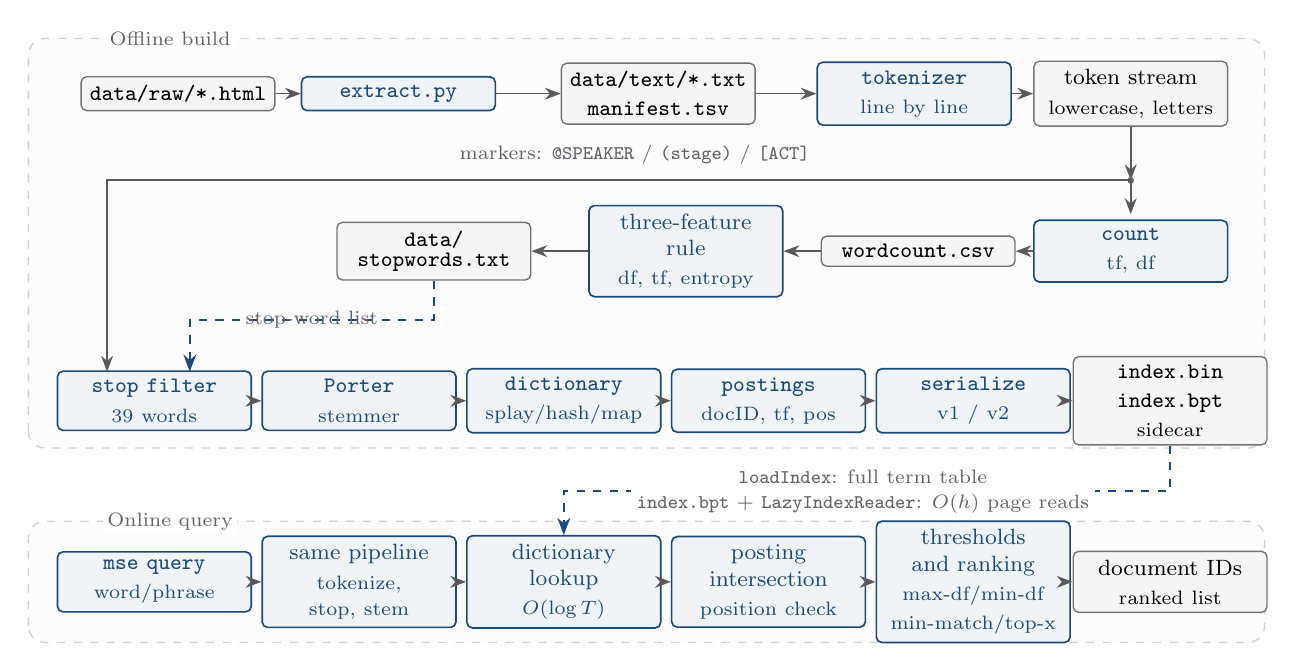
\begin{tikzpicture}[
  font=\footnotesize,
  >=Stealth,
  x=1cm, y=1cm,
  data/.style={draw=black!55, rounded corners=2pt, line width=0.5pt,
               fill=black!4, inner sep=3pt, align=center, text width=2.25cm},
  proc/.style={draw=mseblue, rounded corners=2pt, line width=0.6pt,
               fill=mseblue!6, text=mseblue, inner sep=3pt, align=center,
               text width=2.25cm},
  note/.style={font=\scriptsize, text=msegray, align=center},
  group/.style={draw=black!18, rounded corners=6pt, line width=0.5pt,
                dashed, fill=black!1},
  grouplabel/.style={font=\scriptsize, text=msegray, fill=white,
                     inner sep=1.5pt},
  arr/.style={->, line width=0.6pt, draw=black!65},
  darr/.style={->, dashed, line width=0.7pt, draw=mseblue},
  fork/.style={circle, fill=black!60, inner sep=0pt, minimum size=2.4pt},
]

% ---------------------------------------------------------------- groups
\draw[group] (-0.15,2.65) rectangle (15.55,7.85);
\node[grouplabel] at (1.65,7.85) {Offline build};
\draw[group] (-0.15,0.18) rectangle (15.55,1.72);
\node[grouplabel] at (1.65,1.72) {Online query};

% ---------------------------------------------------------------- corpus
\node[data] (raw) at (1.75,7.15) {\texttt{data/raw/*.html}};
\node[proc] (extract) at (4.55,7.15) {\texttt{extract.py}};
\node[data] (text) at (7.85,7.15) {\texttt{data/text/*.txt}\\[1pt]\texttt{manifest.tsv}};
\node[proc] (tokenizer) at (11.10,7.15) {\texttt{tokenizer}\\[1pt]{\scriptsize line by line}};
\node[data] (tokens) at (13.85,7.15) {token stream\\[1pt]{\scriptsize lowercase, letters}};

\draw[arr] (raw) -- (extract);
\draw[arr] (extract) -- (text);
\draw[arr] (text) -- (tokenizer);
\draw[arr] (tokenizer) -- (tokens);

\node[note] at (7.55,6.38)
  {markers: \texttt{@SPEAKER} / \texttt{(stage)} / \texttt{[ACT]}};

% ---------------------------------------------------------------- fork: count
\coordinate (fork) at (13.85,6.05);
\draw[arr] (tokens.south) -- (fork);
\node[fork] at (fork) {};
\draw[arr] (fork) -- (fork -| 0.85,0) -- (0.85,3.62);

\draw[arr] (fork) -- (13.85,5.62);
\node[proc] (count) at (13.85,5.15) {\texttt{count}\\[1pt]{\scriptsize tf, df}};
\node[data] (wc) at (11.15,5.15) {\texttt{wordcount.csv}};
\node[proc] (rule) at (8.20,5.15) {three-feature\\rule\\[1pt]{\scriptsize df, tf, entropy}};
\node[data] (sw) at (5.00,5.15) {\texttt{data/}\\[-2pt]\texttt{stopwords.txt}};
\draw[arr] (count) -- (wc);
\draw[arr] (wc) -- (rule);
\draw[arr] (rule) -- (sw);

\draw[darr] (sw.south) -- (5.00,4.28) -- (1.90,4.28) -- (1.90,3.62);
\node[note] at (3.45,4.28) {stop-word list};

% ---------------------------------------------------------------- index build
\node[proc] (stop) at (1.45,3.25) {\texttt{stop filter}\\[1pt]{\scriptsize 39 words}};
\node[proc] (stem) at (4.05,3.25) {\texttt{Porter}\\[1pt]{\scriptsize stemmer}};
\node[proc] (dict) at (6.65,3.25) {\texttt{dictionary}\\[1pt]{\scriptsize splay/hash/map}};
\node[proc] (post) at (9.25,3.25) {\texttt{postings}\\[1pt]{\scriptsize docID, tf, pos}};
\node[proc] (ser) at (11.85,3.25) {\texttt{serialize}\\[1pt]{\scriptsize v1 / v2}};
\node[data] (idx) at (14.35,3.25) {\texttt{index.bin}\\[1pt]\texttt{index.bpt}\\[1pt]{\scriptsize sidecar}};

\draw[arr] (stop) -- (stem);
\draw[arr] (stem) -- (dict);
\draw[arr] (dict) -- (post);
\draw[arr] (post) -- (ser);
\draw[arr] (ser) -- (idx);

% ---------------------------------------------------------------- query side
\node[proc] (query) at (1.45,0.95) {\texttt{mse query}\\[1pt]{\scriptsize word/phrase}};
\node[proc] (norm) at (4.05,0.95) {same pipeline\\[1pt]{\scriptsize tokenize, stop, stem}};
\node[proc] (lookup) at (6.65,0.95) {dictionary\\lookup\\[1pt]{\scriptsize $O(\log T)$}};
\node[proc] (intersect) at (9.25,0.95) {posting\\intersection\\[1pt]{\scriptsize position check}};
\node[proc] (thresh) at (11.85,0.95) {thresholds\\and ranking\\[1pt]{\scriptsize max-df/min-df}\\[1pt]{\scriptsize min-match/top-x}};
\node[data] (hits) at (14.35,0.95) {document IDs\\[1pt]{\scriptsize ranked list}};

\draw[arr] (query) -- (norm);
\draw[arr] (norm) -- (lookup);
\draw[arr] (lookup) -- (intersect);
\draw[arr] (intersect) -- (thresh);
\draw[arr] (thresh) -- (hits);

\draw[darr] (idx.south) -- (14.35,2.10) -- (6.65,2.10) -- (lookup.north);
\node[note, fill=white, inner sep=2pt] at (10.45,2.10)
  {\texttt{loadIndex}: full term table\\[1pt]
   \texttt{index.bpt} + \texttt{LazyIndexReader}: $O(h)$ page reads};

\end{tikzpicture}%
}
\caption{System data flow. The offline side extracts the HTML corpus into a
text layer, tokenizes it, removes stop words, applies Porter stemming, and
writes the inverted index; word-frequency counting and stop-word derivation
form a bypass. The online side reuses the same normalization pipeline, then
performs dictionary lookup, posting intersection and position verification,
applies the four thresholds, and returns document IDs. The dashed path is the
B+ tree sidecar written by \code{--dict-file}; a query reads $O(h)$ pages,
where $h$ is the tree height.}
\label{fig:pipeline}
\end{figure}
.
\begin{figure}[!htbp]
\centering
\resizebox{\linewidth}{!}{%
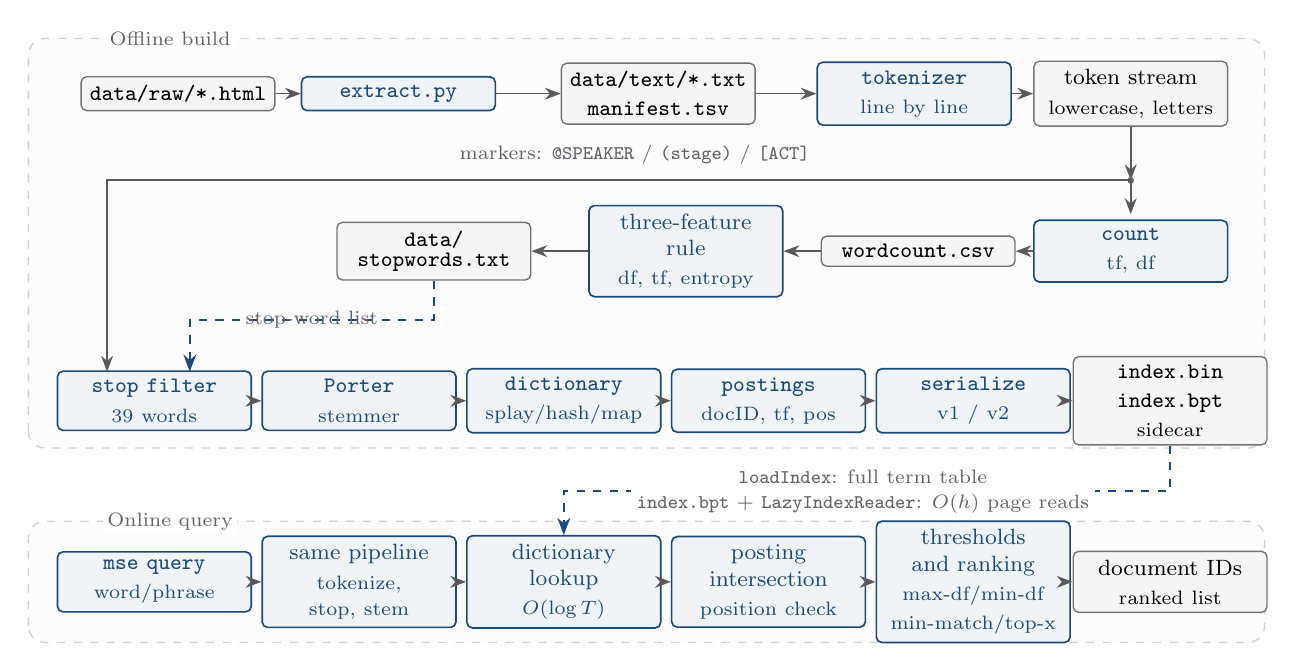
\begin{tikzpicture}[
  font=\footnotesize,
  >=Stealth,
  x=1cm, y=1cm,
  data/.style={draw=black!55, rounded corners=2pt, line width=0.5pt,
               fill=black!4, inner sep=3pt, align=center, text width=2.25cm},
  proc/.style={draw=mseblue, rounded corners=2pt, line width=0.6pt,
               fill=mseblue!6, text=mseblue, inner sep=3pt, align=center,
               text width=2.25cm},
  note/.style={font=\scriptsize, text=msegray, align=center},
  group/.style={draw=black!18, rounded corners=6pt, line width=0.5pt,
                dashed, fill=black!1},
  grouplabel/.style={font=\scriptsize, text=msegray, fill=white,
                     inner sep=1.5pt},
  arr/.style={->, line width=0.6pt, draw=black!65},
  darr/.style={->, dashed, line width=0.7pt, draw=mseblue},
  fork/.style={circle, fill=black!60, inner sep=0pt, minimum size=2.4pt},
]

% ---------------------------------------------------------------- groups
\draw[group] (-0.15,2.65) rectangle (15.55,7.85);
\node[grouplabel] at (1.65,7.85) {Offline build};
\draw[group] (-0.15,0.18) rectangle (15.55,1.72);
\node[grouplabel] at (1.65,1.72) {Online query};

% ---------------------------------------------------------------- corpus
\node[data] (raw) at (1.75,7.15) {\texttt{data/raw/*.html}};
\node[proc] (extract) at (4.55,7.15) {\texttt{extract.py}};
\node[data] (text) at (7.85,7.15) {\texttt{data/text/*.txt}\\[1pt]\texttt{manifest.tsv}};
\node[proc] (tokenizer) at (11.10,7.15) {\texttt{tokenizer}\\[1pt]{\scriptsize line by line}};
\node[data] (tokens) at (13.85,7.15) {token stream\\[1pt]{\scriptsize lowercase, letters}};

\draw[arr] (raw) -- (extract);
\draw[arr] (extract) -- (text);
\draw[arr] (text) -- (tokenizer);
\draw[arr] (tokenizer) -- (tokens);

\node[note] at (7.55,6.38)
  {markers: \texttt{@SPEAKER} / \texttt{(stage)} / \texttt{[ACT]}};

% ---------------------------------------------------------------- fork: count
\coordinate (fork) at (13.85,6.05);
\draw[arr] (tokens.south) -- (fork);
\node[fork] at (fork) {};
\draw[arr] (fork) -- (fork -| 0.85,0) -- (0.85,3.62);

\draw[arr] (fork) -- (13.85,5.62);
\node[proc] (count) at (13.85,5.15) {\texttt{count}\\[1pt]{\scriptsize tf, df}};
\node[data] (wc) at (11.15,5.15) {\texttt{wordcount.csv}};
\node[proc] (rule) at (8.20,5.15) {three-feature\\rule\\[1pt]{\scriptsize df, tf, entropy}};
\node[data] (sw) at (5.00,5.15) {\texttt{data/}\\[-2pt]\texttt{stopwords.txt}};
\draw[arr] (count) -- (wc);
\draw[arr] (wc) -- (rule);
\draw[arr] (rule) -- (sw);

\draw[darr] (sw.south) -- (5.00,4.28) -- (1.90,4.28) -- (1.90,3.62);
\node[note] at (3.45,4.28) {stop-word list};

% ---------------------------------------------------------------- index build
\node[proc] (stop) at (1.45,3.25) {\texttt{stop filter}\\[1pt]{\scriptsize 39 words}};
\node[proc] (stem) at (4.05,3.25) {\texttt{Porter}\\[1pt]{\scriptsize stemmer}};
\node[proc] (dict) at (6.65,3.25) {\texttt{dictionary}\\[1pt]{\scriptsize splay/hash/map}};
\node[proc] (post) at (9.25,3.25) {\texttt{postings}\\[1pt]{\scriptsize docID, tf, pos}};
\node[proc] (ser) at (11.85,3.25) {\texttt{serialize}\\[1pt]{\scriptsize v1 / v2}};
\node[data] (idx) at (14.35,3.25) {\texttt{index.bin}\\[1pt]\texttt{index.bpt}\\[1pt]{\scriptsize sidecar}};

\draw[arr] (stop) -- (stem);
\draw[arr] (stem) -- (dict);
\draw[arr] (dict) -- (post);
\draw[arr] (post) -- (ser);
\draw[arr] (ser) -- (idx);

% ---------------------------------------------------------------- query side
\node[proc] (query) at (1.45,0.95) {\texttt{mse query}\\[1pt]{\scriptsize word/phrase}};
\node[proc] (norm) at (4.05,0.95) {same pipeline\\[1pt]{\scriptsize tokenize, stop, stem}};
\node[proc] (lookup) at (6.65,0.95) {dictionary\\lookup\\[1pt]{\scriptsize $O(\log T)$}};
\node[proc] (intersect) at (9.25,0.95) {posting\\intersection\\[1pt]{\scriptsize position check}};
\node[proc] (thresh) at (11.85,0.95) {thresholds\\and ranking\\[1pt]{\scriptsize max-df/min-df}\\[1pt]{\scriptsize min-match/top-x}};
\node[data] (hits) at (14.35,0.95) {document IDs\\[1pt]{\scriptsize ranked list}};

\draw[arr] (query) -- (norm);
\draw[arr] (norm) -- (lookup);
\draw[arr] (lookup) -- (intersect);
\draw[arr] (intersect) -- (thresh);
\draw[arr] (thresh) -- (hits);

\draw[darr] (idx.south) -- (14.35,2.10) -- (6.65,2.10) -- (lookup.north);
\node[note, fill=white, inner sep=2pt] at (10.45,2.10)
  {\texttt{loadIndex}: full term table\\[1pt]
   \texttt{index.bpt} + \texttt{LazyIndexReader}: $O(h)$ page reads};

\end{tikzpicture}%
}
\caption{System data flow. The offline side extracts the HTML corpus into a
text layer, tokenizes it, removes stop words, applies Porter stemming, and
writes the inverted index; word-frequency counting and stop-word derivation
form a bypass. The online side reuses the same normalization pipeline, then
performs dictionary lookup, posting intersection and position verification,
applies the four thresholds, and returns document IDs. The dashed path is the
B+ tree sidecar written by \code{--dict-file}; a query reads $O(h)$ pages,
where $h$ is the tree height.}
\label{fig:pipeline}
\end{figure}


Keeping the two branches on one tokenizer is a deliberate constraint. It makes
the stop-word list, the stemmer, and the query program share a single
definition of a term, and it lets the index header record the processing flags
so that a query cannot silently use a different normalization.

\subsection{Report Organization}

Chapter~\ref{sec:design} gives the data-structure and algorithm specification,
including pseudo-code for the main operations. Chapter~\ref{sec:results}
presents the test environment, the required test-case table, and the measured
results for the four tasks and the bonus experiments.
Chapter~\ref{sec:analysis} analyzes time and space complexity, compares the
chosen structures with alternatives, generalizes to the RFC corpus, and lists
limitations and improvements. Appendix~\ref{app:source} records the source-code
organization and comment coverage, Appendix~\ref{app:reproduce} gives the
reproduction commands, and Appendix~\ref{app:format} documents the data
formats. The Author List, Declaration, and Signatures follow the appendices.

% Chapter 2: Data structure and algorithm specification.

\section{Data Structure and Algorithm Specification}
\label{sec:design}

This chapter specifies the data structures and algorithms used by the engine.
The order follows the data flow: tokenization, counting, stop-word selection,
stemming, index construction, dictionary structures, disk-based storage,
external construction, and query processing. Pseudo-code is written in a
language-independent form; identifiers such as \code{lastDoc} and
\code{posStart} match the implementation.

\subsection{Tokenization and Normalization}
\label{sec:tokenization}

The corpus is stored as a \emph{text layer}: one semantic unit per line, with a
line marker that identifies headings, stage directions, and speaker labels.
\code{manifest.tsv} is the catalog; each row contains the document ID, title,
text path, and source path, and an optional \code{format} column selects
\code{marked} (default) or \code{plain} (used by the RFC corpus).

A token is a maximal run of ASCII letters that may contain internal
apostrophes. All tokens are lowercased. The apostrophe rules are:

\begin{itemize}
  \item an internal apostrophe is kept: \code{don't} and \code{o'er} are single
        tokens;
  \item a leading apostrophe is dropped: \code{'Tis} becomes \code{tis};
  \item a trailing apostrophe acts as a separator: \code{friends'} becomes
        \code{friends};
  \item hyphens, digits, and ordinary punctuation are separators:
        \code{to-day} becomes \code{to} and \code{day}, and \code{1660s}
        becomes \code{s}.
\end{itemize}

Marker lines are skipped by default. A heading such as \code{[ACT I]}, a stage
direction such as \code{(Exit Ghost)}, or a speaker label such as
\code{@BERNARDO} is recognized only when the first and last characters match
the expected pair. A line that begins with \code{[} but continues as dialogue
is body text. The optional flags \code{--keep-headings}, \code{--keep-speakers},
and \code{--keep-stage} retain each class for experiments that need a different
counting convention.

\begin{lstlisting}[style=cli]
for each line L in the text layer:
    if L is a marker line and the marker class is not kept:
        continue
    for each maximal run T of ASCII letters and internal apostrophes:
        T = drop leading apostrophe; T = lowercase(T)
        emit T
\end{lstlisting}

Normalization is the composition of three stages: tokenize, optionally remove
stop words, and optionally apply the Porter stemmer. The index header stores
two flags for the latter two stages, and the query program reads these flags
and replays the same composition. This is the mechanism that keeps a query
from using a different definition of a term than the index.

\subsection{Word Frequency Statistics}
\label{sec:count-design}

\subsubsection{Design Principles}

For a term $t$, the engine reports its term frequency and document frequency:
\begin{equation}
  \mathrm{tf}(t)=\sum_{d}\mathrm{tf}(t,d),\qquad
  \mathrm{df}(t)=|\{d:\mathrm{tf}(t,d)>0\}|.
\end{equation}
It also computes the document-frequency ratio
$\mathrm{df\_ratio}(t)=\mathrm{df}(t)/195$ and the term-frequency share
$\mathrm{tf\_share}(t)=\mathrm{tf}(t)/866\,626$. The first measures coverage;
the second measures volume. Looking at only one of them makes a dialogue word
diluted by the 154 short poems look rare when it is actually common.

The counter reuses the formal normalization pipeline. Four configurations are
supported: the default (no stop words, no stemming), stop words only, stemming
only, and the formal configuration (both). The same order---tokenize, filter,
stem---is used by the index and query programs.

\subsubsection{Algorithm}

Documents are scanned in manifest order. Each term row stores its accumulated
frequency and the ID of the last document in which it was seen. The document
frequency is incremented only when the current document ID differs from
\code{lastDoc}; repeated occurrences inside one document therefore contribute
once to df.

\begin{lstlisting}[style=cli]
for each document d in manifest order:
    for each token t in tokenize(d):
        row = table[t]
        row.tf += 1
        if row.lastDoc != d.id:
            row.df += 1
            row.lastDoc = d.id
\end{lstlisting}

With a hash table the expected time is $O(N)$ for $N$ tokens, plus $O(T\log T)$
for sorting the output rows; with a splay dictionary it is $O(N\log T)$
amortized. The memory bound is $O(T)$ rows. The four CSV outputs are
deterministic: the same input and flags produce the same bytes, and the files
contain no timestamps.

\subsection{Stop-Word Selection}
\label{sec:stopwords}

\subsubsection{The tf/df Candidate Rule}

The simplest candidate rule asks a word to be both widespread and frequent:
\begin{equation}
  \mathrm{df\_ratio}(t)\ge 0.75
  \quad\land\quad
  \mathrm{tf\_share}(t)\ge 0.001.
\end{equation}
It returns only nine words. The reason is the corpus composition: 154 short
poems account for 79\% of the documents, and many function words do not appear
in every poem, so their document-frequency ratios are diluted. For example,
\code{a} has a ratio of 0.7077, just below 0.75. Lowering the threshold to 0.40
produces 48 candidates, but content words such as \code{love} and \code{time}
enter the band as well.

\subsubsection{Length-Normalized Rate Entropy}
\label{sec:entropy}

To separate ``spread evenly across many documents'' from ``merely frequent,''
the engine computes a length-normalized rate entropy. Let $L_d$ be the number
of kept tokens in document $d$:
\begin{equation}
  r_{t,d}=\frac{\mathrm{tf}(t,d)}{L_d},\qquad
  q_{t,d}=\frac{r_{t,d}}{\sum_{d'}r_{t,d'}},\qquad
  \widehat H(t)=\frac{-\sum_{d}q_{t,d}\log_2 q_{t,d}}{\log_2\mathrm{df}(t)}.
  \label{eq:rate-entropy}
\end{equation}
After length normalization, function words sit above 0.95, content words such
as \code{love}, \code{king}, and \code{heart} are visibly lower, and a proper
noun with $\mathrm{df}=1$ has entropy zero by definition. The denominator
$\log_2\mathrm{df}(t)$ makes the statistic comparable across words that occur
in different numbers of documents.

\subsubsection{The Three-Feature Rule}

The final rule requires a word to be wide, heavy, and flat:
\begin{equation}
  \mathrm{df\_ratio}\ge r
  \quad\land\quad
  \mathrm{tf\_share}\ge s
  \quad\land\quad
  \widehat H\ge h.
\end{equation}
The default $(r,s,h)=(0.75,0.001,0.93)$ yields nine words. The experimental
configuration $(0.40,0.001,0.93)$ yields 39 words and overlaps the manually
curated list in 35 words. The automatic list adds \code{hath}, \code{o},
\code{thee}, and \code{thou}, and omits \code{more}, \code{or}, \code{than},
and \code{their}; each difference can be explained by the rate entropy.

\begin{lstlisting}[style=cli]
for each term t in the vocabulary:
    if df_ratio[t] >= r and tf_share[t] >= s
       and rate_entropy[t] >= h:
        emit t
\end{lstlisting}

The rule is deterministic and uses no external stop-word list. Changing a
threshold changes only the strictness of the band, not the structure of the
rule.

\subsection{Porter Stemming}
\label{sec:stemmer}

\subsubsection{Comparison of Public Stemmers}

Four public descriptions were compared: the original Porter (1980) paper, the
canonical C implementation on the author's site, the NLTK
\code{PorterStemmer} in its three compatibility modes, and the Snowball Porter2
algorithm \cite{porter1980,porter-c,nltk,snowball}. The implementation follows
the 1980 paper plus the three marked \code{--DEPARTURE--} changes in the
canonical C code: words of two letters or fewer are left unchanged, \code{bli}
is changed to \code{ble}, and \code{logi} is changed to \code{log}. This is the
same behavior as NLTK's \code{MARTIN_EXTENSIONS} mode, which the full-vocabulary
cross-check uses as an oracle.

\subsubsection{Algorithm}

Before the Porter rules, contractions are reduced: the longest matching suffix
among \code{n't}, \code{'s}, \code{'d}, \code{'ll}, \code{'re}, \code{'ve},
\code{'t}, and \code{'m} is removed, and remaining apostrophes are deleted.
Thus \code{o'er} becomes \code{oer}, \code{marry'd} becomes \code{marryd}, and
the irregular forms keep their rule result, for example \code{can't} becomes
\code{ca} and \code{won't} becomes \code{wo}.

The main flow executes steps 1a, 1b, 1c, 2, 3, 4, 5a, and 5b. The core
condition is the measure $m$ (the number of vowel-consonant sequences) and the
predicates \code{*v*}, \code{*d}, and \code{*o}. The implementation follows
``the first matching suffix decides'': once a suffix matches, only that rule's
condition is checked; if the condition fails, the step stops and does not fall
back to a shorter suffix. This detail matters: an earlier version continued to
shorter suffixes after a failed condition, over-stemmed 41 word forms (for
example, \code{agreement} became \code{agreem}), and was caught by the
full-vocabulary differential test.

\begin{lstlisting}[style=cli]
stem(word):
    word = strip_longest_contraction(word)
    for step in (1a, 1b, 1c, 2, 3, 4, 5a, 5b):
        for suffix in step.suffixes_by_length:
            if word ends with suffix:
                if step.condition(word, suffix):
                    word = step.replace(word, suffix)
                break          # first match wins; do not try shorter suffixes
    return word
\end{lstlisting}

The worst-case cost is $O(L^2)$ for a word of length $L$ because suffix
matching and condition checks rescan the word; in practice $L$ is small and the
observed throughput is dominated by the dictionary, not by the stemmer.

\subsection{Inverted Index}
\label{sec:posting}

\subsubsection{Posting Lists and Invariants}

Each term has a posting list ordered by document ID. A posting entry stores
$(\mathrm{docID},\mathrm{posStart},\mathrm{tf})$, where \code{posStart} is the
start of the entry's positions in a separate position array and \code{tf} is
the number of occurrences in that document. Positions are offsets in the
stop-word-filtered token stream, so a phrase query can verify adjacency without
returning to the original text.

The loader checks five structural invariants: document IDs are dense from 1 to
$N$; document IDs within one posting list are strictly increasing; the
\code{tf} of each entry equals its number of positions; the total number of
positions equals the total number of kept tokens; and the term table is in
strict lexicographic order. The same invariants are enforced by
\code{validateIndex()} after loading.

\subsubsection{Build Algorithm}

The builder scans the document stream and appends postings incrementally; at
the end, the dictionary is frozen into a sorted term table.

\begin{lstlisting}[style=cli]
for each document D in manifest order:
    pos = 0
    for each token t in tokenize(D):
        if stop_words.contains(t): continue
        term = stem(t) if stem_flag else t
        dict.upsert(term).append(D.id, pos)
        pos += 1
    index.docs.push({D.id, D.title, pos})
index.terms = dict.sorted_entries()
\end{lstlisting}

The formal configuration produces 14,937 terms, 117,704 posting entries,
556,866 positions, and a 3,685,655-byte v1 index. The file layout is shown in
Figure~\ref{fig:index-layout}.

% figures/index-layout.tex -- sequential index layout and posting structure.
% Pure TikZ diagram: field names and byte widths come from include/index.hpp
% and the v1 serializer in src/index.cpp (28 B header, 12+len doc entry,
% 28+len term entry, 8+4*tf posting entry). No measured values.
\begin{figure}[!htbp]
\centering
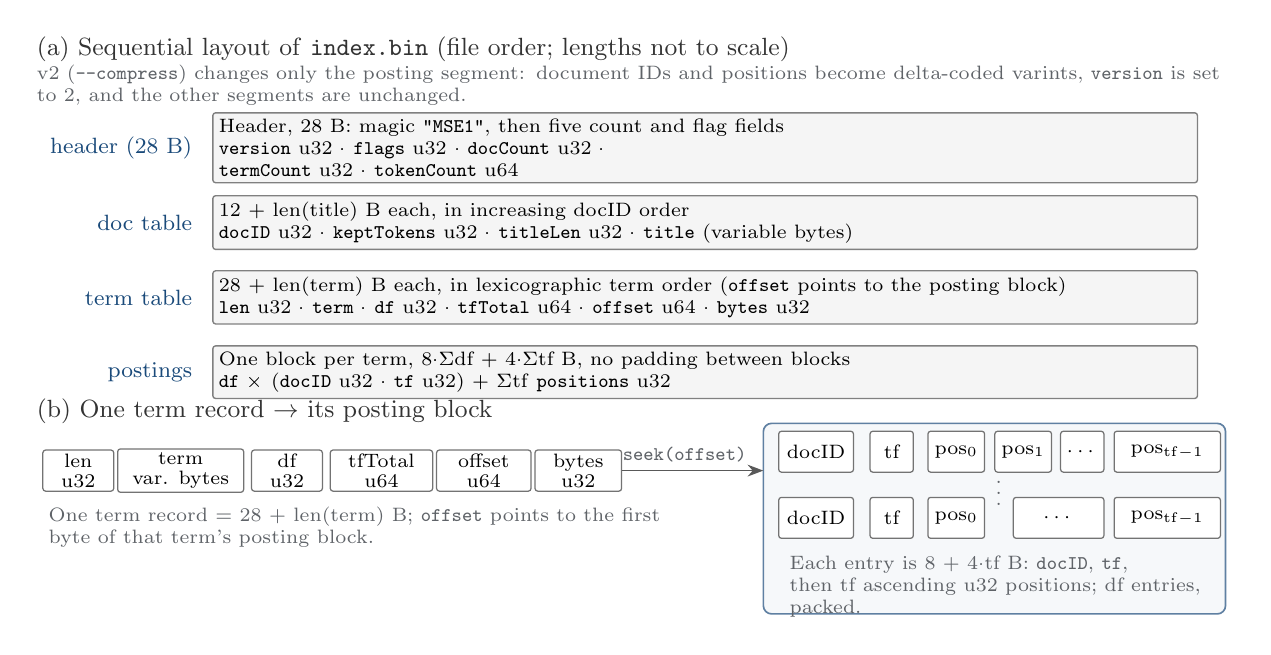
\begin{tikzpicture}[
  font=\footnotesize,
  >=Stealth,
  x=1cm, y=1cm,
  seglabel/.style={font=\footnotesize, text=mseblue, anchor=east},
  strip/.style={draw=black!50, rounded corners=1pt, line width=0.5pt,
                fill=black!4, anchor=west, align=left, inner sep=2.2pt,
                font=\scriptsize, text width=12.35cm},
  cell/.style={draw=black!55, rounded corners=1pt, line width=0.45pt,
               fill=white, align=center, inner sep=1.5pt,
               minimum height=0.52cm, font=\scriptsize},
  structbox/.style={draw=mseblue!70, rounded corners=3pt, line width=0.6pt,
                    fill=mseblue!4},
  title/.style={font=\small, text=black!80, anchor=west, align=left,
                text width=15.2cm},
  note/.style={font=\scriptsize, text=msegray, anchor=west, align=left},
]

% ======================================================= (a) sequential layout
\node[title] at (0.20,7.55)
  {(a) Sequential layout of \texttt{index.bin} (file order; lengths not to
   scale)};
\node[note, text width=15.2cm] at (0.20,7.10)
  {v2 (\texttt{-{}-compress}) changes only the posting segment: document IDs
   and positions become delta-coded varints, \texttt{version} is set to 2, and
   the other segments are unchanged.};

% --- header
\node[seglabel] at (2.42,6.30) {header (28 B)};
\node[strip] at (2.55,6.30)
  {Header, 28 B: magic \texttt{"MSE1"}, then five count and flag fields\\
   \texttt{version} u32 · \texttt{flags} u32 · \texttt{docCount} u32 ·\\
   \texttt{termCount} u32 · \texttt{tokenCount} u64};
% --- document table
\node[seglabel] at (2.42,5.35) {doc table};
\node[strip] at (2.55,5.35)
  {12 + len(title) B each, in increasing docID order\\
   \texttt{docID} u32 · \texttt{keptTokens} u32 · \texttt{titleLen} u32 ·
   \texttt{title} (variable bytes)};
% --- term table
\node[seglabel] at (2.42,4.40) {term table};
\node[strip] at (2.55,4.40)
  {28 + len(term) B each, in lexicographic term order
   (\texttt{offset} points to the posting block)\\
   \texttt{len} u32 · \texttt{term} · \texttt{df} u32 · \texttt{tfTotal} u64 ·
   \texttt{offset} u64 · \texttt{bytes} u32};
% --- postings
\node[seglabel] at (2.42,3.45) {postings};
\node[strip] at (2.55,3.45)
  {One block per term, 8·$\Sigma$df + 4·$\Sigma$tf B, no padding between
   blocks\\
   \texttt{df} × (\texttt{docID} u32 · \texttt{tf} u32) + $\Sigma$tf
   \texttt{positions} u32};

% ======================================================= (b) term -> block
\node[title] at (0.20,2.95)
  {(b) One term record $\rightarrow$ its posting block};

% --- term record: six field cells, byte width on the second line
\node[cell, minimum width=0.90cm] (len) at (0.85,2.20) {len\\[-1pt]{\scriptsize u32}};
\node[cell, minimum width=1.60cm] (term) at (2.15,2.20) {term\\[-1pt]{\scriptsize var. bytes}};
\node[cell, minimum width=0.90cm] (df) at (3.50,2.20) {df\\[-1pt]{\scriptsize u32}};
\node[cell, minimum width=1.30cm] (tftotal) at (4.70,2.20) {tfTotal\\[-1pt]{\scriptsize u64}};
\node[cell, minimum width=1.20cm] (offset) at (6.00,2.20) {offset\\[-1pt]{\scriptsize u64}};
\node[cell, minimum width=1.10cm] (bytes) at (7.20,2.20) {bytes\\[-1pt]{\scriptsize u32}};

\node[note, text width=7.90cm] at (0.35,1.48)
  {One term record = 28 + len(term) B; \texttt{offset} points to the first byte
   of that term's posting block.};

% --- posting block (two records shown; all fields are u32)
\draw[structbox] (9.55,0.38) rectangle (15.42,2.80);

\node[cell, minimum width=0.95cm] at (10.22,2.44) {docID};
\node[cell, minimum width=0.55cm] at (11.18,2.44) {tf};
\node[cell, minimum width=0.72cm] at (12.00,2.44) {pos$_0$};
\node[cell, minimum width=0.72cm] at (12.85,2.44) {pos$_1$};
\node[cell, minimum width=0.55cm] at (13.60,2.44) {$\cdots$};
\node[cell, minimum width=1.35cm] at (14.68,2.44) {pos$_{\mathrm{tf}-1}$};
\node[font=\scriptsize, text=msegray] at (12.54,2.02) {$\vdots$};
\node[cell, minimum width=0.95cm] at (10.22,1.60) {docID};
\node[cell, minimum width=0.55cm] at (11.18,1.60) {tf};
\node[cell, minimum width=0.72cm] at (12.00,1.60) {pos$_0$};
\node[cell, minimum width=1.15cm] at (13.30,1.60) {$\cdots$};
\node[cell, minimum width=1.35cm] at (14.68,1.60) {pos$_{\mathrm{tf}-1}$};

\node[note, anchor=north west, text width=5.40cm] at (9.76,1.24)
  {Each entry is 8 + 4·tf B: \texttt{docID}, \texttt{tf},\\
   then tf ascending u32 positions; df entries, packed.};

% --- term record -> posting block
\draw[->, line width=0.6pt, draw=black!65]
  (bytes.east) -- (9.55,2.20);
\node[note, anchor=south, inner sep=1pt] at (8.55,2.26) {\texttt{seek(offset)}};

\end{tikzpicture}
\caption{Index layout: \texttt{index.bin} stores the header, document table,
term table, and posting segment in order. A term record points to its posting
block with \texttt{offset} and \texttt{bytes}. Within a block, each posting
stores the document ID and term frequency followed by tf ascending positions,
so a phrase query only needs to compare adjacent positions.}
\label{fig:index-layout}
\end{figure}


\subsubsection{Persistence Formats v1 and v2}
\label{sec:persistence}

Persistence is part of the index specification, not an afterthought. Format v1
writes the header, document table, term table, and posting blocks in order. All
offsets are computed before writing, and the reader parses the same layout and
replays the invariant checks. The same index object therefore always produces
the same byte sequence.

Format v2 changes only the posting region: document IDs are stored as deltas,
positions as deltas, and frequencies and deltas use a 1--4 byte byte-aligned
variable-length code. The header, document table, and term table are unchanged,
except that \code{version} is set to 2. On the formal index, v2 reduces
3,685,655 bytes to 1,725,694 bytes, or 46.82\% of v1, with identical query
output.

The variable-length code uses the top two bits of the first byte for the total
length and stores 6, 14, 22, or 30 payload bits in 1, 2, 3, or 4 bytes,
respectively. Values are little-endian. A document-ID delta is at least 1; a
position delta is at least 0.

\subsection{Dictionary Structures}
\label{sec:dict}

The build-time dictionary exposes three operations: \code{upsert},
\code{find}, and \code{sortedEntries}. The primary implementation is a
self-implemented splay tree; a hash table and \code{std::map} are alternative
implementations used for comparison.

\subsubsection{Splay Tree}

The workload explains the choice. The index is insert-only, so the expensive
deletion cases of a red-black tree never occur. The token stream is
Zipf-distributed, and splaying an accessed node to the root keeps frequent terms
near the top. At the end of the build, an in-order traversal produces the sorted
term table directly, which is exactly the frozen dictionary the serializer
needs. The amortized cost of an operation is $O(\log T)$ for $T$ terms; the
worst case is $O(T)$ for a single operation.

\subsubsection{Hash Table and \texttt{std::map}}

The hash dictionary provides expected $O(1)$ lookup and no ordered traversal;
it is the speed baseline. The \code{std::map} dictionary is a red-black tree
with worst-case $O(\log T)$ lookup and stable behavior; it is the balanced-tree
control. Both implement the same three-operation interface, and all three
produce byte-identical index files. The comparison of their build costs is
reported in Section~\ref{sec:dict-analysis}.

\subsubsection{Comparison}

The splay tree pays for its ordered traversal with rotations and a higher
comparison count; the hash table is faster but cannot produce a sorted term
list without an extra sort; \code{std::map} sits between them with predictable
costs. None of these differences changes the persisted index, because the
dictionary is frozen before serialization.

\subsection{Disk-Based B+ Tree}
\label{sec:bptree-design}

For a vocabulary that does not fit in memory, the query side can use a disk B+
tree \emph{sidecar} that maps each term to its posting offset and block length.
The tree is a 4\,KiB page file: page 0 is the header, and each later page is a
leaf or an inner node. Leaves are linked by \code{nextLeaf} in key order. Keys
are variable-length strings; the fanout is determined by the byte budget.

The value of a leaf entry is a 64-bit integer that packs the posting block
offset and the block length:
\begin{equation}
  \mathrm{value}=(\mathrm{offset}\ll 21)\;|\;\mathrm{blockBytes}.
\end{equation}
The length field is 21 bits, which is ample for the block sizes in this
project.

The tree maintains five invariants, checked by \code{validate()}. The routing
interval is left-closed, $[\mathrm{key}_{i-1},\mathrm{key}_i)$, because a
separator key is a real copy of the smallest key in the right subtree. With
variable-length keys, a count-based split does not guarantee a 50\% byte fill;
the implementation splits at the byte midpoint of a legal window and uses the
provable lower bound \code{pageSize/2 - maxEntry} for the fill check. A lookup
reads the root-to-leaf path and then seeks to the posting block:

\begin{lstlisting}[style=cli]
page = readPage(root)
while page is an inner node:
    i = upper_bound(page.keys, key)   # left-closed intervals
    page = readPage(page.child[i])
binary search page.keys for key
if found: return page.value
else: return not_found
\end{lstlisting}

A lookup costs $O(h)$ page reads and $O(h\log F)$ comparisons for height $h$
and fanout $F$; it does not load the full term table. The sidecar is built by
bulk-loading the sorted terms and is rebuilt whenever the index is rebuilt.

\subsection{Block-Based External Construction}
\label{sec:spimi}

The in-memory builder keeps the whole dictionary and all postings in memory.
For a large corpus this is the wrong bound, so the project also implements a
SPIMI-style block builder. Documents are streamed one at a time; the buffer is
spilled to a sorted temporary \emph{run} when it reaches a term budget
(\code{--block-terms}) or an estimated byte budget (\code{--block-bytes}). Runs
are then merged in passes with at most \code{--merge-fan-in} inputs per pass.
The term metadata and postings are streamed to temporary files and assembled
into the final index, so the process does not rebuild the full index or all
compressed blocks in memory.

\begin{lstlisting}[style=cli]
for each document D in manifest order:
    add tokens of D to buffer
    if buffer.terms >= term_budget or buffer.bytes >= byte_budget:
        sort buffer; write run; clear buffer
if buffer is non-empty: sort buffer; write run
merge runs in passes of at most fan_in runs
\end{lstlisting}

The memory bound is the block budget plus document metadata, run paths, file
buffers, and one document. The budget is checked at document boundaries, so a
single document can exceed it. Because every run boundary falls between
documents, document IDs increase across runs, and the postings of the same term
can be concatenated during the merge without reordering.

On the Shakespeare corpus with a budget of 4,096, the builder produces 17 runs,
peaks at 5,129 live terms, writes 4,166,556 bytes of temporary run data, and
produces an index byte-identical to the in-memory build. The merge cost is
$O(T\cdot R)$ with a linear scan of all run cursors, or $O(T\log R)$ with a heap;
the implementation uses the simpler scan and reports the cost in
Section~\ref{sec:compression}.

\subsection{Query Processing and Threshold Design}
\label{sec:query-design}

\subsubsection{Normalization Pipeline}

The query text is tokenized, filtered, and stemmed by the same functions used at
build time. The index header flags decide whether stop-word filtering and
stemming are applied. Every term that is filtered, missing from the dictionary,
or dropped by a threshold is reported in an explanatory message, so an empty
result is not silent.

\subsubsection{Word, Phrase, and Boolean Queries}

A word query must normalize to exactly one term. A multi-word query uses
\code{--words}; a phrase query uses \code{--phrase}. For a phrase, the engine
starts from the term with the smallest document frequency, takes its documents
as candidates, and verifies that the remaining terms occur at
\code{start+1}, \code{start+2}, and so on. Positions are sorted, so each check
is a binary search.

\begin{lstlisting}[style=cli]
phrase_query(terms):
    choose t0 with the smallest df
    for each document d in postings(t0):
        for each start position p of t0 in d:
            if for every i in 1..k-1: p+i is in positions(t_i, d):
                emit d; break
\end{lstlisting}

A Boolean query requires all searchable terms by default. The score vector is
\code{(matched, tfSum, docID)}, sorted by descending matched count, descending
term-frequency sum, and ascending document ID, which makes the result order
deterministic. \code{--min-match k} requires at least $k$ matching terms; if
$k$ exceeds the number of searchable terms, it is clamped to that number.

\subsubsection{Thresholds}

All four thresholds act at query time; the index is built once. Their positions
and defaults are listed in Table~\ref{tab:threshold-params}.

\begin{table}[!ht]
  \centering
  \caption{Query thresholds: where they act and their defaults.}
  \label{tab:threshold-params}
  \small
  \begin{tabularx}{\linewidth}{l l l X}
    \toprule
    Option & Default & Stage & Meaning \\
    \midrule
    \code{--max-df} & 1.0 & query-term filter & drop a term whose df ratio exceeds the threshold \\
    \code{--min-df} & 1 & query-term filter & drop a term whose df is below the threshold \\
    \code{--min-match} & 0 & Boolean condition & require at least $k$ matching terms; 0 means all \\
    \code{--top-x} & 0 & result truncation & keep only the first $x$ documents after ranking \\
    \bottomrule
  \end{tabularx}
\end{table}

Phrase queries deliberately bypass \code{--max-df} and \code{--min-df}: a phrase
must match as a whole, and dropping any term changes its meaning. A query whose
terms are all stop words always returns nothing, because stop words never enter
the index; the program distinguishes ``stop word'' from ``not in the
dictionary'' in its explanation.

\subsection{Summary of Main Data Structures}
\label{sec:data-structures}

Table~\ref{tab:data-structures} summarizes the structures that carry the
invariants and costs discussed above. The table is a specification reference;
measured numbers appear in Chapter~\ref{sec:results}.

\begin{table}[!htbp]
  \centering
  \caption{Main data structures, invariants, and operation costs.}
  \label{tab:data-structures}
  \footnotesize
  \renewcommand{\arraystretch}{1.05}
  \begin{tabularx}{\linewidth}{@{}l X X X@{}}
    \toprule
    Structure & Key fields / layout & Invariants & Operations and cost \\
    \midrule
    Posting entry &
      \code{docID} u32, \code{posStart} u32, \code{tf} u32 &
      document IDs strictly increasing; \code{tf} equals the number of
      positions &
      append $O(1)$; phrase check $O(\log \mathrm{tf})$ per position \\
    Document table &
      \code{docID}, \code{keptTokens}, \code{title} &
      IDs dense from 1 to $N$; \code{keptTokens} sums to the total positions &
      lookup by ID $O(1)$ \\
    Splay dictionary &
      term, posting block, left/right child &
      binary-search-tree order; splay moves the accessed node to the root &
      \code{upsert}/\code{find} $O(\log T)$ amortized, $O(T)$ worst;
      \code{sortedEntries} $O(T)$ \\
    Hash dictionary &
      term, posting block, bucket array &
      load factor bounded; rehash preserves entries &
      expected $O(1)$ lookup; no ordered traversal \\
    B+ tree node &
      leaf flag, \code{keyCount}, \code{nextLeaf}, keys, values/children &
      left-closed routing intervals; byte fill lower bound; leaf chain in key
      order &
      lookup $O(h)$ page reads and $O(h\log F)$ comparisons \\
    Index header &
      \code{magic}, \code{version}, \code{flags}, \code{docCount},
      \code{termCount}, \code{tokenCount} &
      flags replay the build-time normalization; counts match the tables &
      read once $O(1)$ \\
    Block run &
      sorted sequence of (term, partial postings) &
      runs are disjoint by document range; document IDs increase across runs &
      merge $O(T\log R)$ with a heap, $O(TR)$ with a linear scan \\
    \bottomrule
  \end{tabularx}
\end{table}

% =====================================================================
% 第 3 章 测试与结果（owner: writer-results）
%
% 数字来源约定（均为本轮 2026-10-20 重新构建/重新运行的结果）：
%   % src: tasks F##  —— reports/data/results-tasks.md（任务 1–3 实测，F1–F42）
%   % src: verify F## —— reports/data/results-verify.md（测试/交叉验证/Bonus，F1–F18）
%   % src: pre P##    —— reports/data/results-preprocess.md（预处理复核，P1–P6）
% 本章不使用 README.md/notes.md/plan.md 里的历史数字；开发期 bug 只作定性叙述，
% 修复后的验证结论一律取本轮实测结果。每个表格/段落前标注其证据编号。
% =====================================================================

\newpage
\section{测试与结果分析}
\label{sec:results}

% 本章有 14 张表、3 张图，局部收紧缩放间距，减少浮动体造成的整页空白；
% 章末恢复 article 默认值，避免影响后续章节。
\setlength{\textfloatsep}{8pt plus 2pt minus 2pt}
\setlength{\floatsep}{8pt plus 2pt minus 2pt}
\setlength{\intextsep}{8pt plus 2pt minus 2pt}

\subsection{词频统计与停用词选择}

\subsubsection{词频统计结果}
\label{sec:wordcount}

默认配置只统计正文行。195 个文档共切分出 866\,626 个词元，其中不同词项
25\,705 个，仅出现一次的词项 9\,753 个。核心统计量见表~\ref{tab:wordcount}。

\begin{table}[!htbp]
  \centering
  \caption{默认配置下的词频统计结果}
  \label{tab:wordcount}
  \small
  \begin{tabular}{lr}
    \toprule
    指标 & 数值 \\
    \midrule
    文档数 & 195 \\
    正文词元数 & 866\,626 \\
    不同词项数 & 25\,705 \\
    仅出现一次的词项数 & 9\,753 \\
    \bottomrule
  \end{tabular}
\end{table}

默认配置下词频最高的 10 个词项见表~\ref{tab:top10}。
% src: tasks F7
\begin{table}[!htbp]
  \centering
  \caption{默认配置下词频最高的 10 个词项（含文档频率与两种占比）}
  \label{tab:top10}
  \footnotesize
  \renewcommand{\arraystretch}{1.0}
  \begin{tabular}{r l r r r r}
    \toprule
    排名 & 词项 & 词频 & 文档频率 & 文档频率比值 & 词频占比 \\
    \midrule
    1 & \code{the} & 28\,436 & 177 & 0.9077 & 0.032812 \\
    2 & \code{and} & 25\,553 & 189 & 0.9692 & 0.029486 \\
    3 & \code{i}   & 21\,131 & 154 & 0.7897 & 0.024383 \\
    4 & \code{to}  & 20\,302 & 187 & 0.9590 & 0.023426 \\
    5 & \code{of}  & 16\,976 & 175 & 0.8974 & 0.019589 \\
    6 & \code{a}   & 14\,527 & 138 & 0.7077 & 0.016763 \\
    7 & \code{you} & 13\,998 & 75  & 0.3846 & 0.016152 \\
    8 & \code{my}  & 12\,934 & 159 & 0.8154 & 0.014925 \\
    9 & \code{that}& 11\,513 & 172 & 0.8821 & 0.013285 \\
    10& \code{in}  & 11\,479 & 181 & 0.9282 & 0.013246 \\
    \bottomrule
  \end{tabular}
  \par\smallskip
  \footnotesize 注：文档频率比值为文档频率/195，词频占比为词频/866\,626；数值取自  % src: tasks F7
  \code{wordcount-default.csv} 的权威副本。
\end{table}

% figures/zipf.tex -- 词频—排名分布（双对数），Zipf 定律
%
% 数据：reports/data/csv/tasks/wordcount-default.csv（本轮 mse count，默认管线）
% 由 figures/data/make_figures_data.py 生成 figures/data/zipf.dat 与 zipf-meta.tex。
% 主文档只写 % figures/zipf.tex -- 词频—排名分布（双对数），Zipf 定律
%
% 数据：reports/data/csv/tasks/wordcount-default.csv（本轮 mse count，默认管线）
% 由 figures/data/make_figures_data.py 生成 figures/data/zipf.dat 与 zipf-meta.tex。
% 主文档只写 \input{figures/zipf}。
\input{figures/data/zipf-meta}
\begin{figure}[!htbp]
\centering
\begin{tikzpicture}
\begin{axis}[
  width=0.94\linewidth, height=6.0cm,
  xmode=log, ymode=log,
  xmin=1, xmax=40000, ymin=1, ymax=1e5,
  xlabel={rank (log scale)}, ylabel={term frequency tf (log scale)},
  xtick={1,10,100,1000,10000},
  ytick={1,10,100,1000,10000},
  tick label style={font=\scriptsize},
  label style={font=\small},
  grid=major, grid style={black!8},
  legend style={draw=none, fill=none, font=\scriptsize,
                at={(0.98,0.98)}, anchor=north east},
  legend cell align=left,
]
  % 实测 tf(rank)
  \addplot[only marks, mark=*, mark size=1.0pt, color=mseblue]
    table[x=rank, y=tf] {figures/data/zipf.dat};
  \addlegendentry{measured tf (\ZipfTerms{} terms)}
  % 1/rank 参考线（按 rank 1 处缩放对齐）
  \addplot[dashed, line width=0.8pt, color=msegray]
    table[x=rank, y=ref] {figures/data/zipf.dat};
  \addlegendentry{$1/\mathrm{rank}$ reference (scaled at rank 1)}
  % 最频词标注
  \node[font=\scriptsize, text=msegray, anchor=west] (topword)
    at (axis cs:1.15,42000) {the};
  \draw[->, draw=msegray, line width=0.4pt] (topword.west) -- (axis cs:1.0,3.1e4);
  % hapax 尾标注
  \node[font=\scriptsize, text=msegray, align=left, anchor=south west]
    at (rel axis cs:0.02,0.03)
    {hapax tail: \ZipfHapax{} terms (\ZipfHapaxPct\% of vocabulary)\\
     occur exactly once (tf $=1$)};
\end{axis}
\end{tikzpicture}
\caption{莎士比亚语料的词频—排名分布（双对数）：实测点近似一条直线，符合
Zipf 定律；\ZipfTerms{} 个词中有 \ZipfHapax{} 个只出现一次（占词表
\ZipfHapaxPct\%），构成需要倒排索引兜住的长尾。}%
\label{fig:zipf}
\end{figure}
。
% zipf-meta.tex -- generated by figures/data/make_figures_data.py
\newcommand{\ZipfTerms}{25\,705}
\newcommand{\ZipfHapax}{9\,753}
\newcommand{\ZipfHapaxPct}{37.9}

\begin{figure}[!htbp]
\centering
\begin{tikzpicture}
\begin{axis}[
  width=0.94\linewidth, height=6.0cm,
  xmode=log, ymode=log,
  xmin=1, xmax=40000, ymin=1, ymax=1e5,
  xlabel={rank (log scale)}, ylabel={term frequency tf (log scale)},
  xtick={1,10,100,1000,10000},
  ytick={1,10,100,1000,10000},
  tick label style={font=\scriptsize},
  label style={font=\small},
  grid=major, grid style={black!8},
  legend style={draw=none, fill=none, font=\scriptsize,
                at={(0.98,0.98)}, anchor=north east},
  legend cell align=left,
]
  % 实测 tf(rank)
  \addplot[only marks, mark=*, mark size=1.0pt, color=mseblue]
    table[x=rank, y=tf] {figures/data/zipf.dat};
  \addlegendentry{measured tf (\ZipfTerms{} terms)}
  % 1/rank 参考线（按 rank 1 处缩放对齐）
  \addplot[dashed, line width=0.8pt, color=msegray]
    table[x=rank, y=ref] {figures/data/zipf.dat};
  \addlegendentry{$1/\mathrm{rank}$ reference (scaled at rank 1)}
  % 最频词标注
  \node[font=\scriptsize, text=msegray, anchor=west] (topword)
    at (axis cs:1.15,42000) {the};
  \draw[->, draw=msegray, line width=0.4pt] (topword.west) -- (axis cs:1.0,3.1e4);
  % hapax 尾标注
  \node[font=\scriptsize, text=msegray, align=left, anchor=south west]
    at (rel axis cs:0.02,0.03)
    {hapax tail: \ZipfHapax{} terms (\ZipfHapaxPct\% of vocabulary)\\
     occur exactly once (tf $=1$)};
\end{axis}
\end{tikzpicture}
\caption{莎士比亚语料的词频—排名分布（双对数）：实测点近似一条直线，符合
Zipf 定律；\ZipfTerms{} 个词中有 \ZipfHapax{} 个只出现一次（占词表
\ZipfHapaxPct\%），构成需要倒排索引兜住的长尾。}%
\label{fig:zipf}
\end{figure}


前十个词几乎全是功能词，合计占 20.41\% 的词元。图~\ref{fig:zipf} 的双对数曲线
进一步显示，高频词集中在曲线左端，绝大多数词项位于右端的低频长尾。仅出现一次的词
占到全部词项的 37.94\%，却只覆盖 1.125\% 的词元，说明语料具有明显的“短词表头部、
长低频尾部”特征。由此不能仅凭词频高低判断停用词，下一步还需要比较文档覆盖范围和
文档间分布。

\subsubsection{停用词选择结果}
\label{sec:stopword-results}

% src: tasks F10、F11
表~\ref{tab:candidates} 是候选规则对文档频率阈值的敏感性扫描：固定词频占比
$\ge 0.001$，把文档频率比值阈值从 0.90 降到 0.40。
\begin{table}[!htbp]
  \centering
  \caption{停用词候选带对文档频率比值阈值的敏感性（固定词频占比 $\ge 0.001$）}
  \label{tab:candidates}
  \footnotesize
  \renewcommand{\arraystretch}{1.0}
  \begin{tabularx}{\linewidth}{c c c X}
    \toprule
    文档频率比值阈值 $T$ & 候选数 & 相对上一档新增 & 新增词 \\
    \midrule
    0.90 & 4  & --- & \code{the and to in} \\
    0.75 & 9  & +5  & \code{i of my that but} \\
    0.70 & 14 & +5  & \code{a is not for with} \\
    0.65 & 16 & +2  & \code{so love} \\
    0.60 & 21 & +5  & \code{me be thou thy thee} \\
    0.50 & 31 & +10 & \code{it this as by all do on from which when} \\
    0.40 & 48 & +17 & \code{his have what no if are o or more then their hath than yet mine time doth} \\
    \bottomrule
  \end{tabularx}
  \par\smallskip
  \footnotesize 注：规则为文档频率比值 $\ge T$ 且词频占比 $\ge 0.001$；静态 39 词表就是  % src: tasks F11
  在 0.40 档 48 词候选带上人工取舍的结果。
\end{table}

0.75 档只有 9 个纯功能词；0.65 档内容词 \code{love} 进入候选（文档频率比值 0.651）；0.40
档就混入 \code{time}、\code{thou/thee} 等不该删除的词。纯统计规则能可靠框出"最像
停用词"的一小段，却无法自己决定线的位置——静态表是在 48 词候选带上人工保留结构性
功能词的结果，下一节用速率熵自动完成同一步。

\subsubsection{自动推导结果}

两特征候选带把最后一步留给人工审核；加上"平"（速率熵）后，规则能否自动得到与人工表
几乎相同的停用词？表~\ref{tab:stopword-sweep} 是四组阈值与 39 词静态表的双向差集。
% src: tasks F13、F14
\begin{table}[!htbp]
  \centering
  \caption{三特征停用词推导的阈值扫描：与静态 39 词表的差异}
  \label{tab:stopword-sweep}
  \footnotesize
  \renewcommand{\arraystretch}{1.0}
  \begin{tabularx}{\linewidth}{c c c c X}
    \toprule
    (文档频率比值, 速率熵) & 推导词数 & 重叠 & 静态表独有 & 推导表独有 \\
    \midrule
    (0.75, 0.93) & 9  & 9  & 30 & --- \\
    (0.50, 0.95) & 23 & 23 & 16 & --- \\
    (0.40, 0.93) & 39 & 35 & \code{more or than their} & \code{hath o thee thou} \\
    (0.30, 0.93) & 50 & 35 & \code{more or than their} & \code{at hath he him how let now o thee there thou was well would you} \\
    \bottomrule
  \end{tabularx}
  \par\smallskip
  \footnotesize 注：词频占比固定为 $\ge 0.001$，文档频率比值取第一列；  % src: tasks F13
  (0.75,0.93) 档 9 词与两特征候选带一致，(0.40,0.93) 档复现静态表所在的 39 词带。
\end{table}

(0.40, 0.93) 档推导出 39 词、与静态表重叠 35 个；差异恰好是 4 对可解释的词：自动
推导多收 \code{hath o thee thou} 四个古体功能词，静态表多收 \code{more or than
their} 四个兼作比较、并列用的词。前者在原文本中同样"宽而平"，后者是人工按语义判断的
取舍。也就是说，三特征规则把"是不是停用词"从人工经验变成可复算的判定，结果与人工表
只差 4 个词且差异可逐词解释；换一档阈值只改变严格度（9/23/39/50 词），不改变规则
结构。四个输出文件都带出处头且不含时间戳，换参数可以直接重跑比较。

图~\ref{fig:entropy} 把功能词、内容词与专名的速率熵画成条形图并标出 0.93 阈值线。

% figures/entropy.tex -- 速率熵（entropy_rate_norm）判别停用词
%
% 数据：reports/data/csv/tasks/wordcount-default.csv（本轮 mse count，默认管线）
% 由 figures/data/make_figures_data.py 生成 figures/data/entropy-*.dat。
% 主文档只写 % figures/entropy.tex -- 速率熵（entropy_rate_norm）判别停用词
%
% 数据：reports/data/csv/tasks/wordcount-default.csv（本轮 mse count，默认管线）
% 由 figures/data/make_figures_data.py 生成 figures/data/entropy-*.dat。
% 主文档只写 \input{figures/entropy}。
\begin{figure}[!htbp]
\centering
\begin{tikzpicture}
\begin{axis}[
  width=0.96\linewidth, height=5.3cm,
  ymin=0, ymax=1.06,
  ytick={0,0.2,0.4,0.6,0.8,1.0},
  ylabel={entropy\_rate\_norm},
  symbolic x coords={the,and,i,to,of,is,it,that,love,king,heart,sweet,man,osric,banquo},
  xtick={the,and,i,to,of,is,it,that,love,king,heart,sweet,man,osric,banquo},
  xticklabel style={font=\scriptsize, rotate=40, anchor=north east, inner sep=1pt},
  tick label style={font=\scriptsize},
  label style={font=\small},
  enlarge x limits=0.04,
  grid=major, grid style={black!8},
  legend columns=4,
  legend style={at={(0.5,-0.23)}, anchor=north, draw=none, font=\scriptsize},
  legend cell align=left,
]
  % 功能词：速率熵接近 1
  \addplot[ycomb, color=mseblue, line width=1.0pt,
           mark=*, mark size=1.8pt, mark options={fill=mseblue}]
    table[x=term, y=rate] {figures/data/entropy-function.dat};
  \addlegendentry{function words}
  % 内容词：明显偏低
  \addplot[ycomb, color=msegray, line width=0.9pt,
           mark=square*, mark size=1.6pt, mark options={fill=msegray}]
    table[x=term, y=rate] {figures/data/entropy-content.dat};
  \addlegendentry{content words}
  % 专名：df=1 时按定义为 0
  \addplot[ycomb, color=black!35, line width=0.9pt,
           mark=triangle*, mark size=2.0pt, mark options={fill=black!35}]
    table[x=term, y=rate] {figures/data/entropy-name.dat};
  \addlegendentry{proper nouns (df $=1$)}
  % 规则阈值 0.93
  \addplot[dashed, line width=0.8pt, color=black!65, mark=none]
    table[x=term, y=threshold] {figures/data/entropy-threshold.dat};
  \addlegendentry{0.93 threshold}
\end{axis}
\end{tikzpicture}
\caption{速率熵判别：功能词全部贴近 1（均在 0.96 以上），专名（df${}=1$）
按定义为 0，内容词落在 0.83–0.94 的低区间；0.93 一条横线即可把功能词与其余
词分开，个别越线的内容词再被 df 比例门（$\ge 0.4$）挡住，说明该特征能替代
人工逐个审核。}%
\label{fig:entropy}
\end{figure}
。
\begin{figure}[!htbp]
\centering
\begin{tikzpicture}
\begin{axis}[
  width=0.96\linewidth, height=5.3cm,
  ymin=0, ymax=1.06,
  ytick={0,0.2,0.4,0.6,0.8,1.0},
  ylabel={entropy\_rate\_norm},
  symbolic x coords={the,and,i,to,of,is,it,that,love,king,heart,sweet,man,osric,banquo},
  xtick={the,and,i,to,of,is,it,that,love,king,heart,sweet,man,osric,banquo},
  xticklabel style={font=\scriptsize, rotate=40, anchor=north east, inner sep=1pt},
  tick label style={font=\scriptsize},
  label style={font=\small},
  enlarge x limits=0.04,
  grid=major, grid style={black!8},
  legend columns=4,
  legend style={at={(0.5,-0.23)}, anchor=north, draw=none, font=\scriptsize},
  legend cell align=left,
]
  % 功能词：速率熵接近 1
  \addplot[ycomb, color=mseblue, line width=1.0pt,
           mark=*, mark size=1.8pt, mark options={fill=mseblue}]
    table[x=term, y=rate] {figures/data/entropy-function.dat};
  \addlegendentry{function words}
  % 内容词：明显偏低
  \addplot[ycomb, color=msegray, line width=0.9pt,
           mark=square*, mark size=1.6pt, mark options={fill=msegray}]
    table[x=term, y=rate] {figures/data/entropy-content.dat};
  \addlegendentry{content words}
  % 专名：df=1 时按定义为 0
  \addplot[ycomb, color=black!35, line width=0.9pt,
           mark=triangle*, mark size=2.0pt, mark options={fill=black!35}]
    table[x=term, y=rate] {figures/data/entropy-name.dat};
  \addlegendentry{proper nouns (df $=1$)}
  % 规则阈值 0.93
  \addplot[dashed, line width=0.8pt, color=black!65, mark=none]
    table[x=term, y=threshold] {figures/data/entropy-threshold.dat};
  \addlegendentry{0.93 threshold}
\end{axis}
\end{tikzpicture}
\caption{速率熵判别：功能词全部贴近 1（均在 0.96 以上），专名（df${}=1$）
按定义为 0，内容词落在 0.83–0.94 的低区间；0.93 一条横线即可把功能词与其余
词分开，个别越线的内容词再被 df 比例门（$\ge 0.4$）挡住，说明该特征能替代
人工逐个审核。}%
\label{fig:entropy}
\end{figure}


功能词 the、and、i、to、of、is、it、that 的速率熵都在 0.95 以上（the 0.9748、
and 0.9789），内容词 love、king、heart、sweet 落在 0.82--0.93（0.9271、0.8260、
0.8313、0.8925），只出现在一篇文档的专名 osric、banquo 按定义为 0。0.93 的线正好切在
功能词与内容词之间；\code{man} 的速率熵 0.9388 略高于阈值线，但文档频率比值只有 0.2359，
被"宽"这一条件挡在候选带外——三个条件是"与"关系，速率熵补上的正是前两个特征缺失的
"分布是否均匀"这一维。

最终停用词的选择是 \code{the and i to of a my that in is not me it for with be his this but have as so what by no all do if are on from or which more then their when than yet}。

\subsection{倒排索引与查询结果}

\subsubsection{倒排索引构建结果}
\label{sec:index-build}

正式倒排索引采用 39 词停用表并执行词干化。构建完成后的结果见
表~\ref{tab:index-configs}。
% src: tasks F18、F21
\begin{table}[!htbp]
  \centering
  \caption{正式倒排索引的最终构建结果}
  \label{tab:index-configs}
  \small
  \begin{tabular}{lr}
    \toprule
    指标 & 结果 \\
    \midrule
    文档数 & 195 \\
    保留词元数 & 556\,866 \\
    词项数 & 14\,937 \\
    倒排记录数 & 117\,704 \\
    位置数 & 556\,866 \\
    第一版索引大小 & 3\,685\,655 字节 \\
    第二版索引大小 & 1\,725\,694 字节 \\
    构建时间 & 0.19\,秒 \\
    \bottomrule
  \end{tabular}
\end{table}

表~\ref{tab:dict-compare} 比较三种词典实现构建同一份正式索引时的代价。
% src: tasks F20
\begin{table}[!htbp]
  \centering
  \caption{三种词典实现的构建代价（正式配置，各构建 3 次）}
  \label{tab:dict-compare}
  \footnotesize
  \renewcommand{\arraystretch}{1.0}
  \begin{tabular}{l r r r l}
    \toprule
    词典 & 比较次数 & 旋转次数 & 再哈希次数 & 构建时间（内建 / 外部中位） \\
    \midrule
    伸展树（主） & 6\,392\,724 & 5\,850\,795 & 0 & 0.19\,s / 0.2610\,s \\
    哈希表 & 688\,494 & 0 & 11 & 0.09\,s / \textbf{0.1603\,s} \\
    \code{std::map}（对照） & 9\,435\,694 & 0 & 0 & 0.14\,s / 0.2084\,s \\
    \bottomrule
  \end{tabular}
  \par\smallskip
  \footnotesize 注：比较次数、旋转次数、再哈希次数为 C++ 内建计数；外部墙钟含进程  % src: tasks F20
  启动与文件读写，受并行负载影响只作量级比较。
\end{table}

从构建速度看，哈希表最快，标准映射次之，伸展树最慢；从字符串比较次数看，哈希表也
明显少于两种树结构。伸展树的主要代价是 585 万次旋转，但它的中序遍历可以直接得到
有序词项表。项目因此以伸展树作为主词典，以哈希表作为速度基线，以标准映射作为平衡树
对照。第二版索引在第一版基础上降至 172 万字节，约为原来的 46.82\%。

\subsubsection{查询结果}
\label{sec:query}

本节使用正式索引测试单词、短语和布尔查询，并检查无结果时能否说明原因。
代表性查询见表~\ref{tab:query-examples}。
% src: tasks F27–F33
\begin{table}[!htbp]
  \centering
  \caption{正式索引上的代表性查询结果}
  \label{tab:query-examples}
  \footnotesize
  \renewcommand{\arraystretch}{1.0}
  \begin{tabularx}{\linewidth}{l l r X}
    \toprule
    查询 & 类型 & 文档数 & 结果说明 \\
    \midrule
    \code{osric} & 单词 & 1 & 文档 30《Hamlet》，可定位到原句 \\
    \code{love} & 单词 & 138 & 高频内容词，返回全部包含该词的文档 \\
    \code{good night} & 短语 & 23 & 两个词必须位置相邻 \\
    \code{king richard} & 短语 & 7 & 两个词均存在并通过位置验证 \\
    \code{my lord} & 短语 & 42 & \code{my} 被停用词过滤，实际只查 \code{lord} \\
    \code{to be or not to be} & 短语 & 0 & 全部由停用词组成 \\
    \code{king queen} & 布尔 & 33 & 默认要求两个词全部命中 \\
    \code{the} & 单词 & 0 & 停用词未进入索引 \\
    \code{notaword} & 单词 & 0 & 索引词典中没有该词 \\
    \bottomrule
  \end{tabularx}
\end{table}

单词查询直接返回包含目标词项的文档编号和标题。结果按命中词数、词频总和和文档编号
稳定排序。加上 \code{--pretty} 后，程序会重新运行文本处理管线，在结果中附上词语
所在的原句，便于核对命中位置。

短语查询要验证多个词项在过滤停用词后的词元序列中连续出现，不能只求两个倒排记录表
的交集。\code{good night} 命中 23 篇，只有两个词完整相邻出现的文档会被保留。由于
位置定义在过滤后的词元序列上，\code{my lord} 中的 \code{my} 不占位置，系统实际执行
的是 \code{lord} 的单词查询。全部由停用词组成的短语没有可定位的词项，因此返回空结果。

布尔查询默认要求所有查询词都命中。\code{king queen} 因此返回 33 篇；使用
\code{--min-match 1} 后只需命中任意一个词，结果增加到 43 篇。无结果时，程序会区分
“停用词未进入索引”和“索引词典中没有该词”，避免把所有空结果混为一类。

\subsection{阈值实验与复杂度分析}

\subsubsection{阈值实验结果}
\label{sec:threshold}

四个参数都只作用于查询。全部关闭时，同一查询的结果作为基线。实验每次只改变一个参数，
共选 15 条查询，覆盖高频词、中频词、低频词、专名、普通短语、含停用词短语、布尔查询
和停用词。对全部查询测试 5 档最大文档频率、4 档最小文档频率和 3 档结果截断；最少
命中词数只适用于 king queen 与 sweet sword moon 两条布尔查询，取 3 档。由此得到
$15+15\times(5+4+3)+2\times3=201$ 条测量。每条记录返回数、相对基线的 Jaccard
相似度、说明信息条数和耗时，全部使用同一份正式索引。图~\ref{fig:threshold} 展示了
四个参数对返回文档数的影响。

% figures/threshold.tex -- 四个查询阈值对返回文档数的影响（2x2 面板）
%
% 数据：reports/data/csv/tasks/threshold_matrix.csv（本轮 tools/threshold_matrix.py
% 的 201 条测量；off 行即无阈值基线）。由 figures/data/make_figures_data.py
% 生成 figures/data/threshold-*.dat。主文档只写 % figures/threshold.tex -- 四个查询阈值对返回文档数的影响（2x2 面板）
%
% 数据：reports/data/csv/tasks/threshold_matrix.csv（本轮 tools/threshold_matrix.py
% 的 201 条测量；off 行即无阈值基线）。由 figures/data/make_figures_data.py
% 生成 figures/data/threshold-*.dat。主文档只写 \input{figures/threshold}。
\pgfplotsset{
  % 面板公共设置
  figthaxis/.style={
    width=7.10cm, height=2.90cm,
    ymin=0,
    xtick style={draw=black!40},
    tick label style={font=\scriptsize},
    label style={font=\small},
    title style={font=\small},
    grid=major, grid style={black!8},
    unbounded coords=discard,
  },
  % 每条查询一条曲线：颜色/线型/标记三者组合区分
  figthlove/.style={color=mseblue, line width=0.9pt, mark=*, mark size=1.1pt},
  figthsword/.style={color=mseblue, dashed, line width=0.9pt,
                     mark=square*, mark size=1.0pt},
  figthphrase/.style={color=msegray, line width=0.9pt,
                      mark=triangle*, mark size=1.3pt},
  figthkq/.style={color=msegray, dashed, line width=0.9pt,
                  mark=diamond*, mark size=1.1pt},
  figthssm/.style={color=black!65, densely dotted, line width=1.0pt,
                   mark=o, mark size=1.1pt},
}
\begin{figure}[!htbp]
\centering
\captionsetup[subfigure]{font=scriptsize,skip=2pt}
% ---------------- (a) max-df ----------------
\begin{subfigure}{0.49\linewidth}
  \centering
  \begin{tikzpicture}
  \begin{axis}[figthaxis,
    xlabel={max-df threshold}, ylabel={result documents},
    xtick={0,1,2,3,4,5}, xticklabels={0.1,0.3,0.5,0.7,0.9,off},
    xmin=-0.55, xmax=5.55,
    legend to name={figthresholdlegend}, legend columns=3,
    legend style={draw=none, font=\scriptsize},
  ]
    \addplot[figthlove] table[x=idx, y=love] {figures/data/threshold-max-df.dat};
    \addlegendentry{love (word)}
    \addplot[figthsword] table[x=idx, y=sword] {figures/data/threshold-max-df.dat};
    \addlegendentry{sword (word)}
    \addplot[figthphrase] table[x=idx, y=kr_phrase] {figures/data/threshold-max-df.dat};
    \addlegendentry{king richard (phrase)}
    \addplot[figthkq] table[x=idx, y=kq_bool] {figures/data/threshold-max-df.dat};
    \addlegendentry{king queen (bool)}
    \addplot[figthssm] table[x=idx, y=ssm_bool] {figures/data/threshold-max-df.dat};
    \addlegendentry{sweet sword moon (bool)}
  \end{axis}
  \end{tikzpicture}
  \caption{max-df：裁掉 df 比例过高的查询词}
\end{subfigure}\hfill
% ---------------- (b) min-df ----------------
\begin{subfigure}{0.49\linewidth}
  \centering
  \begin{tikzpicture}
  \begin{axis}[figthaxis,
    xlabel={min-df threshold},
    xtick={0,1,2,3,4}, xticklabels={off,2,5,20,50},
    xmin=-0.55, xmax=4.55,
  ]
    \addplot[figthlove, forget plot] table[x=idx, y=love] {figures/data/threshold-min-df.dat};
    \addplot[figthsword, forget plot] table[x=idx, y=sword] {figures/data/threshold-min-df.dat};
    \addplot[figthphrase, forget plot] table[x=idx, y=kr_phrase] {figures/data/threshold-min-df.dat};
    \addplot[figthkq, forget plot] table[x=idx, y=kq_bool] {figures/data/threshold-min-df.dat};
    \addplot[figthssm, forget plot] table[x=idx, y=ssm_bool] {figures/data/threshold-min-df.dat};
  \end{axis}
  \end{tikzpicture}
  \caption{min-df：按文档频率下限裁词}
\end{subfigure}

\vspace{0.15em}
% ---------------- (c) min-match ----------------
\begin{subfigure}{0.49\linewidth}
  \centering
  \begin{tikzpicture}
  \begin{axis}[figthaxis,
    xlabel={min-match $k$}, ylabel={result documents},
    xtick={0,1,2}, xticklabels={1,2,3},
    xmin=-0.55, xmax=2.55,
  ]
    % 只有布尔查询有 min-match 数据（词/短语查询没有 k-of-n 语义）
    \addplot[figthkq, forget plot] table[x=idx, y=kq_bool] {figures/data/threshold-min-match.dat};
    \addplot[figthssm, forget plot] table[x=idx, y=ssm_bool] {figures/data/threshold-min-match.dat};
  \end{axis}
  \end{tikzpicture}
  \caption{min-match：要求命中 $k$ 个查询词（仅布尔查询）}
\end{subfigure}\hfill
% ---------------- (d) top-x ----------------
\begin{subfigure}{0.49\linewidth}
  \centering
  \begin{tikzpicture}
  \begin{axis}[figthaxis,
    xlabel={top-x cap},
    xtick={0,1,2}, xticklabels={5,10,20},
    xmin=-0.55, xmax=2.55,
  ]
    \addplot[figthlove, forget plot] table[x=idx, y=love] {figures/data/threshold-top-x.dat};
    \addplot[figthsword, forget plot] table[x=idx, y=sword] {figures/data/threshold-top-x.dat};
    \addplot[figthphrase, forget plot] table[x=idx, y=kr_phrase] {figures/data/threshold-top-x.dat};
    \addplot[figthkq, forget plot] table[x=idx, y=kq_bool] {figures/data/threshold-top-x.dat};
    \addplot[figthssm, forget plot] table[x=idx, y=ssm_bool] {figures/data/threshold-top-x.dat};
  \end{axis}
  \end{tikzpicture}
  \caption{top-x：只截断结果条数}
\end{subfigure}

\par\smallskip
\pgfplotslegendfromname{figthresholdlegend}
\caption{四个阈值改变的是查询语义而非结果数量：max-df/min-df 裁掉查询词
（单词查询结果可在临界档归零，双词语句裁词后结果反而变多），min-match 改
布尔条件，top-x 只截断条数；短语查询对前两个参数不敏感。}%
\label{fig:threshold}
\end{figure}
。
\pgfplotsset{
  % 面板公共设置
  figthaxis/.style={
    width=7.10cm, height=2.90cm,
    ymin=0,
    xtick style={draw=black!40},
    tick label style={font=\scriptsize},
    label style={font=\small},
    title style={font=\small},
    grid=major, grid style={black!8},
    unbounded coords=discard,
  },
  % 每条查询一条曲线：颜色/线型/标记三者组合区分
  figthlove/.style={color=mseblue, line width=0.9pt, mark=*, mark size=1.1pt},
  figthsword/.style={color=mseblue, dashed, line width=0.9pt,
                     mark=square*, mark size=1.0pt},
  figthphrase/.style={color=msegray, line width=0.9pt,
                      mark=triangle*, mark size=1.3pt},
  figthkq/.style={color=msegray, dashed, line width=0.9pt,
                  mark=diamond*, mark size=1.1pt},
  figthssm/.style={color=black!65, densely dotted, line width=1.0pt,
                   mark=o, mark size=1.1pt},
}
\begin{figure}[!htbp]
\centering
\captionsetup[subfigure]{font=scriptsize,skip=2pt}
% ---------------- (a) max-df ----------------
\begin{subfigure}{0.49\linewidth}
  \centering
  \begin{tikzpicture}
  \begin{axis}[figthaxis,
    xlabel={max-df threshold}, ylabel={result documents},
    xtick={0,1,2,3,4,5}, xticklabels={0.1,0.3,0.5,0.7,0.9,off},
    xmin=-0.55, xmax=5.55,
    legend to name={figthresholdlegend}, legend columns=3,
    legend style={draw=none, font=\scriptsize},
  ]
    \addplot[figthlove] table[x=idx, y=love] {figures/data/threshold-max-df.dat};
    \addlegendentry{love (word)}
    \addplot[figthsword] table[x=idx, y=sword] {figures/data/threshold-max-df.dat};
    \addlegendentry{sword (word)}
    \addplot[figthphrase] table[x=idx, y=kr_phrase] {figures/data/threshold-max-df.dat};
    \addlegendentry{king richard (phrase)}
    \addplot[figthkq] table[x=idx, y=kq_bool] {figures/data/threshold-max-df.dat};
    \addlegendentry{king queen (bool)}
    \addplot[figthssm] table[x=idx, y=ssm_bool] {figures/data/threshold-max-df.dat};
    \addlegendentry{sweet sword moon (bool)}
  \end{axis}
  \end{tikzpicture}
  \caption{max-df：裁掉 df 比例过高的查询词}
\end{subfigure}\hfill
% ---------------- (b) min-df ----------------
\begin{subfigure}{0.49\linewidth}
  \centering
  \begin{tikzpicture}
  \begin{axis}[figthaxis,
    xlabel={min-df threshold},
    xtick={0,1,2,3,4}, xticklabels={off,2,5,20,50},
    xmin=-0.55, xmax=4.55,
  ]
    \addplot[figthlove, forget plot] table[x=idx, y=love] {figures/data/threshold-min-df.dat};
    \addplot[figthsword, forget plot] table[x=idx, y=sword] {figures/data/threshold-min-df.dat};
    \addplot[figthphrase, forget plot] table[x=idx, y=kr_phrase] {figures/data/threshold-min-df.dat};
    \addplot[figthkq, forget plot] table[x=idx, y=kq_bool] {figures/data/threshold-min-df.dat};
    \addplot[figthssm, forget plot] table[x=idx, y=ssm_bool] {figures/data/threshold-min-df.dat};
  \end{axis}
  \end{tikzpicture}
  \caption{min-df：按文档频率下限裁词}
\end{subfigure}

\vspace{0.15em}
% ---------------- (c) min-match ----------------
\begin{subfigure}{0.49\linewidth}
  \centering
  \begin{tikzpicture}
  \begin{axis}[figthaxis,
    xlabel={min-match $k$}, ylabel={result documents},
    xtick={0,1,2}, xticklabels={1,2,3},
    xmin=-0.55, xmax=2.55,
  ]
    % 只有布尔查询有 min-match 数据（词/短语查询没有 k-of-n 语义）
    \addplot[figthkq, forget plot] table[x=idx, y=kq_bool] {figures/data/threshold-min-match.dat};
    \addplot[figthssm, forget plot] table[x=idx, y=ssm_bool] {figures/data/threshold-min-match.dat};
  \end{axis}
  \end{tikzpicture}
  \caption{min-match：要求命中 $k$ 个查询词（仅布尔查询）}
\end{subfigure}\hfill
% ---------------- (d) top-x ----------------
\begin{subfigure}{0.49\linewidth}
  \centering
  \begin{tikzpicture}
  \begin{axis}[figthaxis,
    xlabel={top-x cap},
    xtick={0,1,2}, xticklabels={5,10,20},
    xmin=-0.55, xmax=2.55,
  ]
    \addplot[figthlove, forget plot] table[x=idx, y=love] {figures/data/threshold-top-x.dat};
    \addplot[figthsword, forget plot] table[x=idx, y=sword] {figures/data/threshold-top-x.dat};
    \addplot[figthphrase, forget plot] table[x=idx, y=kr_phrase] {figures/data/threshold-top-x.dat};
    \addplot[figthkq, forget plot] table[x=idx, y=kq_bool] {figures/data/threshold-top-x.dat};
    \addplot[figthssm, forget plot] table[x=idx, y=ssm_bool] {figures/data/threshold-top-x.dat};
  \end{axis}
  \end{tikzpicture}
  \caption{top-x：只截断结果条数}
\end{subfigure}

\par\smallskip
\pgfplotslegendfromname{figthresholdlegend}
\caption{四个阈值改变的是查询语义而非结果数量：max-df/min-df 裁掉查询词
（单词查询结果可在临界档归零，双词语句裁词后结果反而变多），min-match 改
布尔条件，top-x 只截断条数；短语查询对前两个参数不敏感。}%
\label{fig:threshold}
\end{figure}


% src: tasks F37、F38、F39
表~\ref{tab:threshold-rows} 按参数归并代表性读数。
\begin{table}[!htbp]
  \centering
  \caption{四个查询阈值对返回结果的影响}
  \label{tab:threshold-rows}
  \footnotesize
  \renewcommand{\arraystretch}{1.0}
  \begin{tabular}{l l l c}
    \toprule
    参数 & 代表查询 & 取值：基线 $\to$ 结果 & Jaccard \\
    \midrule
    \code{--max-df} & \code{love} & 0.9/0.7：138 $\to$ 138/0 & 1.00/0.00 \\
    \code{--min-df} & \code{sweet sword moon} & 50：30 $\to$ 90 & 0.3333 \\
    \code{--min-match} &
      \makecell[l]{\code{king queen}\\\code{sweet sword moon}} &
      \makecell[l]{1/2/3：33 $\to$ 43/33/33\\1/2/3：30 $\to$ 93/39/30} &
      \makecell[c]{0.7674/1.00/1.00\\0.3226/0.7692/1.00} \\
    \code{--top-x} & \code{love} & 5/10/20：138 $\to$ 5/10/20 &
      0.0362/0.0725/0.1449 \\
    \bottomrule
  \end{tabular}
  \par\smallskip
  \footnotesize 注：Jaccard 为结果文档集合与基线集合的交并比；两个空集视为相同。  % src: tasks F38、F39
\end{table}

最高文档频率和最低文档频率筛选的是查询词，不是命中的文档。单词查询只有一个词项，
所以词项被删后结果会直接归零。love 的文档频率比值为 0.7077，在 0.7 档返回数从
138 降到 0；sweet 的比值为 0.4615，在 0.3 档也降到 0。

多词查询会先失去一项约束。sweet sword moon 的基线是 30 篇，使用
\code{--min-df 50} 后，文档频率为 37 和 35 的 sword、moon 被删，只剩 sweet，
于是三词全部命中退化为单词查询，结果反而增加到 90 篇。这个变化不能解释为“阈值提高了
精度”，它说明词项筛选已经改变了查询本身的含义。

最少命中词数在结果侧控制布尔条件。$k=1$ 相当于并集，$k=2$ 要求至少命中两词，
$k=3$ 对应三词全部命中；当 $k$ 超过可用词数时，程序将其限制为词项数。结果截断的
行为更直接：排序完成后只保留前 $x$ 篇，因此 love 的结果依次变为 5、10、20 篇，
不会改变返回文档之间的相对顺序。

短语和停用词给出了两类边界情况。短语查询绕过最大、最小文档频率阈值，king richard
在所有档上都保持 7 篇；如果删掉其中任何一个词，原短语就不再成立。停用词没有进入
索引，所以 the、of 在任何阈值下都返回 0。201 条测量中有 23 条 Jaccard 为 0，
逐条核对后，它们都发生在所有有效查询词项被删空之后；说明信息也记录了对应词项和
丢弃原因，没有出现无说明的空结果。

\paragraph{结论} 四个阈值并不是同一种“收紧”。最大、最小文档频率改变参与匹配的词项，
最少命中词数改变布尔条件，结果截断只改变输出范围。词项被删后，结果数可能归零，
也可能因为约束被削弱而上升。

\subsubsection{复杂度分析}
\label{sec:complexity}

表~\ref{tab:complexity} 给出主要操作的时间与空间上界。$N$、$T$、$P$、$D$、$H$ 分别
表示词元数、词项数、倒排记录数、文档数和命中文档数；$k$ 是查询词数，$R$ 是临时块数，
$B$ 是块预算，$C$ 是词典比较成本。短语验证中的 $\mathrm{tf}_{\max}$ 表示候选词项
在单个文档内的最大词频。

\begin{table}[!htbp]
  \centering
  \caption{主要操作的时间与空间复杂度上界}
  \label{tab:complexity}
  \footnotesize
  \begin{tabular}{l l l}
    \toprule
    操作 & 时间 & 空间 \\
    \midrule
    建索引（内存） & $O(N+\sum \mathrm{df}\cdot C)$ & $O(T+P+N)$ \\
    建索引（块式） & $O(N+RB\log B+TR)$ &
      $O(B+\text{当前块倒排记录})$ \\
    单词查询 & $O(\log T+\mathrm{df}+H\log H)$ & $O(D)$ \\
    短语查询 &
      $O(\mathrm{df}_{\min}\,\mathrm{tf}_{\max}\,k\log\mathrm{tf}_{\max}+H\log H)$ &
      $O(D+k)$ \\
    布尔查询 & $O(\sum \mathrm{df}+H\log H)$ & $O(D)$ \\
    第二版索引编码 & $O(P+N)$ & $O(\text{单块})$ \\
    B+ 树查找 & $O(h\log F)$，另需 $O(h)$ 次页读 & $O(h)$ 页缓存 \\
    \bottomrule
  \end{tabular}
\end{table}

内存建索引的时间主要花在每个词元的词典访问上，输出部分则同时保存词项表、倒排记录和
位置。三种词典写出的索引大小相同，改变的只是比较次数和比较常数。块式构建用 $B$
限制同时驻留的活词，但不能消掉全部成本：$B$ 越小，临时块越多，排序和归并的代价
越容易显现。磁盘 B+ 树换了一种取舍，查询只读取根到叶的 $O(h)$ 个页，不再要求完整
词项表常驻内存。

查询侧的主要成本是遍历相关倒排记录，以及排序命中文档。短语查询先选文档频率最小的
词项，可以缩小候选集，但仍要对每个候选验证 $k$ 个位置。阈值与复杂度的联系也很直接：
最大、最小文档频率在遍历倒排记录之前删词，可能减少后续工作；最少命中词数和结果截断
发生在计分之后，其中 \code{--top-x} 只减少输出数量，不会省掉扫描和排序。对于当前
实现，阈值首先是改变查询语义的工具，不是统一的性能优化开关。

\setlength{\textfloatsep}{20pt plus 2pt minus 4pt}
\setlength{\floatsep}{12pt plus 2pt minus 2pt}
\setlength{\intextsep}{12pt plus 2pt minus 2pt}

% 3.6 Bonus: scalability experiments.
% Evidence: results-verify.md and results-tasks.md (F11-F15, F21-F22).

\subsection{Bonus: Scalability Experiments}
\label{sec:bonus}

The bonus question has two independent scale axes: 500,000 files stress the
build side and the document table, while 400,000,000 distinct words stress the
dictionary and the posting lists. The project implements three mechanisms for
these axes---SPIMI-style block construction, a disk-based B+ tree dictionary,
and the delta-coded v2 index format---and runs the scale experiments that fit
on one machine.

\subsubsection{Scale Boundaries and Measured Range}
\label{sec:scale-range}

The 500,000-document synthetic corpus contains 4,908,747 distinct terms. Its
full in-memory index peaks at 2.00\,GiB. Scaling that figure linearly by term
count to 400,000,000 distinct words would require about 160\,GiB, which a
single machine of this class cannot provide. An in-memory build therefore
cannot answer the second axis directly.

The file axis is measured end to end: statistics, block construction, and the
in-memory build all run on the same 16\,GiB machine, and no address-space or
document-table problem appears at 500,000 files. The distinct-word axis is not
run end to end. The query side is measured up to 50,000,000 B+ tree keys and
extrapolated from the measured trend; the build side is measured to 4.9
million terms and bounded by the $O(\text{budget})$ memory argument. Measured
points and extrapolated points are labelled as such throughout this section.

\subsubsection{Disk B+ Tree Dictionary}
\label{sec:bptree-results}

The query-side problem is not how to search faster but how to avoid loading
the complete term table. The B+ tree sidecar maps each term to a posting
offset and block length, so a lookup touches only a few pages on the root-to-
leaf path. The experiment measures 100,000 to 50,000,000 keys; results are in
Table~\ref{tab:bptree-scale}.

\begin{table}[!htbp]
  \centering
  \caption{Measured scaling of the B+ tree dictionary (4\,KiB pages, bulk
  load, 1,000 random lookups all verified).}
  \label{tab:bptree-scale}
  \small
  \begin{tabular}{r r r r r r}
    \toprule
    Keys & Height & Pages & File bytes & Bytes/key & Page reads/query \\
    \midrule
    100\,000     & 2 & 369     & 1\,515\,520   & 15.1552 & 2.00 \\
    1\,000\,000   & 3 & 3\,688   & 15\,110\,144  & 15.1101 & 3.00 \\
    10\,000\,000  & 3 & 36\,865  & 151\,003\,136 & 15.1003 & 3.00 \\
    30\,000\,000  & 3 & 110\,593 & 452\,993\,024 & 15.0998 & 3.00 \\
    50\,000\,000  & 4 & 184\,322 & 754\,987\,008 & 15.0997 & 4.00 \\
    \bottomrule
  \end{tabular}
  \par\smallskip
  \footnotesize Note: page reads are the actual number of pages read with a
  one-page cache; they equal the tree height.
\end{table}

% figures/bptree.tex -- B+ 树 词典的规模实验：文件体积与查询页读
%
% 数据：reports/data/csv/verify/bptree-bench.csv（本轮 mse bptree-bench，
% 4 KiB 页；100k/1M/10M/30M/50M 键各一次测量）。由
% figures/data/make_figures_data.py 生成 figures/data/bptree-*.dat 与
% bptree-meta.tex（线性拟合、4 亿键外推）。
% 主文档只写 % figures/bptree.tex -- B+ 树 词典的规模实验：文件体积与查询页读
%
% 数据：reports/data/csv/verify/bptree-bench.csv（本轮 mse bptree-bench，
% 4 KiB 页；100k/1M/10M/30M/50M 键各一次测量）。由
% figures/data/make_figures_data.py 生成 figures/data/bptree-*.dat 与
% bptree-meta.tex（线性拟合、4 亿键外推）。
% 主文档只写 \input{figures/bptree}。
\input{figures/data/bptree-meta}
\begin{figure}[!htbp]
\centering
\captionsetup[subfigure]{font=scriptsize,skip=2pt}
% ---------------- (a) file size ----------------
\begin{subfigure}{0.49\linewidth}
  \centering
  \begin{tikzpicture}
  \begin{axis}[
    width=7.10cm, height=4.25cm,
    xmode=log, ymode=log,
    xmin=8e4, xmax=1e9, ymin=1e6, ymax=3e10,
    xlabel={number of keys (log scale)}, ylabel={file size (log scale)},
    xtick={1e5,1e6,1e7,1e8}, xticklabels={100k,1M,10M,100M},
    extra x ticks={4e8}, extra x tick labels={400M},
    extra x tick style={tick label style={font=\scriptsize}},
    ytick={1e6,1e7,1e8,1e9,1e10},
    yticklabels={1 MB,10 MB,100 MB,1 GB,10 GB},
    tick label style={font=\scriptsize},
    label style={font=\small},
    grid=major, grid style={black!8},
    legend style={draw=none, fill=none, font=\scriptsize,
                  at={(0.02,0.98)}, anchor=north west},
    legend cell align=left,
  ]
    % 实测点
    \addplot[only marks, mark=*, mark size=1.4pt, color=mseblue]
      table[x=keys, y=file_bytes] {figures/data/bptree-size.dat};
    \addlegendentry{measured (4 KiB pages)}
    % 15.1 B/key 线性拟合（对数坐标下为直线）
    \addplot[dashed, line width=0.8pt, color=msegray]
      table[x=keys, y=fit_bytes] {figures/data/bptree-size-fit.dat};
    \addlegendentry{linear fit (\BptSlope{} B/key)}
    % 4 亿键外推点（空心）
    \addplot[only marks, mark=o,
             mark options={draw=mseblue, fill=white, line width=0.7pt},
             mark size=2.2pt]
      table[x=keys, y=fit_bytes] {figures/data/bptree-extrap.dat};
    \addlegendentry{400M-key extrapolation}
  \end{axis}
  \end{tikzpicture}
  \caption{文件字节 $=$ \BptSlope{} B/键 $\times$ 键数，严格线性}
\end{subfigure}\hfill
% ---------------- (b) page reads ----------------
\begin{subfigure}{0.49\linewidth}
  \centering
  \begin{tikzpicture}
  \begin{axis}[
    width=7.10cm, height=4.25cm,
    xmode=log,
    xmin=8e4, xmax=1e9, ymin=0, ymax=5,
    xlabel={number of keys (log scale)},
    ylabel={page reads per lookup},
    xtick={1e5,1e6,1e7,1e8}, xticklabels={100k,1M,10M,100M},
    extra x ticks={4e8}, extra x tick labels={400M},
    extra x tick style={tick label style={font=\scriptsize}},
    ytick={0,1,2,3,4,5},
    tick label style={font=\scriptsize},
    label style={font=\small},
    grid=major, grid style={black!8},
    legend style={draw=none, fill=none, font=\scriptsize,
                  at={(0.02,0.98)}, anchor=north west},
    legend cell align=left,
  ]
    % 实测页读（点旁标树高）
    \addplot[only marks, mark=*, mark size=1.4pt, color=mseblue]
      table[x=keys, y=page_reads] {figures/data/bptree-reads.dat};
    \addlegendentry{measured (h $=$ tree height)}
    % 4 亿键外推（虚线延到空心点）
    \addplot[dashed, line width=0.8pt, color=msegray]
      table[x=keys, y=page_reads] {figures/data/bptree-reads-fit.dat};
    \addlegendentry{extrapolated}
    \addplot[only marks, mark=o,
             mark options={draw=mseblue, fill=white, line width=0.7pt},
             mark size=2.2pt]
      table[x=keys, y=page_reads] {figures/data/bptree-extrap.dat};
    % 外推读数标注（放在数据点下方的空白处）
    \node[font=\scriptsize, text=msegray, align=right, anchor=south east]
      at (rel axis cs:0.98,0.04)
      {\BptExtrapM{}M keys: height \BptExtrapH{},\\
       \BptExtrapPages{} page reads $=$ \BptExtrapKiB{} KiB};
  \end{axis}
  \end{tikzpicture}
  \caption{每次查询只读树高页：4 亿键也只需 4 页 $=$ 16 KiB}
\end{subfigure}
\caption{B+ 树 词典的规模实验：文件体积严格线性（\BptSlope{} B/键），而每次
随机查询的页读等于树高、随高度对数增长；按实测扇外出推，4 亿个不同词只需
\BptExtrapH{} 层、每次查询 \BptExtrapPages{} 页（\BptExtrapKiB{} KiB），文件约
\BptExtrapGB{} GB。}%
\label{fig:bptree}
\end{figure}
。
% bptree-meta.tex -- generated by figures/data/make_figures_data.py
\newcommand{\BptSlope}{15.1}
\newcommand{\BptExtrapM}{400}
\newcommand{\BptExtrapGB}{6.04}
\newcommand{\BptExtrapH}{4}
\newcommand{\BptExtrapPages}{4}
\newcommand{\BptExtrapKiB}{16}
\newcommand{\BptLeafKeys}{271}
\newcommand{\BptFanout}{372}

\begin{figure}[!htbp]
\centering
\captionsetup[subfigure]{font=scriptsize,skip=2pt}
% ---------------- (a) file size ----------------
\begin{subfigure}{0.49\linewidth}
  \centering
  \begin{tikzpicture}
  \begin{axis}[
    width=7.10cm, height=4.25cm,
    xmode=log, ymode=log,
    xmin=8e4, xmax=1e9, ymin=1e6, ymax=3e10,
    xlabel={number of keys (log scale)}, ylabel={file size (log scale)},
    xtick={1e5,1e6,1e7,1e8}, xticklabels={100k,1M,10M,100M},
    extra x ticks={4e8}, extra x tick labels={400M},
    extra x tick style={tick label style={font=\scriptsize}},
    ytick={1e6,1e7,1e8,1e9,1e10},
    yticklabels={1 MB,10 MB,100 MB,1 GB,10 GB},
    tick label style={font=\scriptsize},
    label style={font=\small},
    grid=major, grid style={black!8},
    legend style={draw=none, fill=none, font=\scriptsize,
                  at={(0.02,0.98)}, anchor=north west},
    legend cell align=left,
  ]
    % 实测点
    \addplot[only marks, mark=*, mark size=1.4pt, color=mseblue]
      table[x=keys, y=file_bytes] {figures/data/bptree-size.dat};
    \addlegendentry{measured (4 KiB pages)}
    % 15.1 B/key 线性拟合（对数坐标下为直线）
    \addplot[dashed, line width=0.8pt, color=msegray]
      table[x=keys, y=fit_bytes] {figures/data/bptree-size-fit.dat};
    \addlegendentry{linear fit (\BptSlope{} B/key)}
    % 4 亿键外推点（空心）
    \addplot[only marks, mark=o,
             mark options={draw=mseblue, fill=white, line width=0.7pt},
             mark size=2.2pt]
      table[x=keys, y=fit_bytes] {figures/data/bptree-extrap.dat};
    \addlegendentry{400M-key extrapolation}
  \end{axis}
  \end{tikzpicture}
  \caption{文件字节 $=$ \BptSlope{} B/键 $\times$ 键数，严格线性}
\end{subfigure}\hfill
% ---------------- (b) page reads ----------------
\begin{subfigure}{0.49\linewidth}
  \centering
  \begin{tikzpicture}
  \begin{axis}[
    width=7.10cm, height=4.25cm,
    xmode=log,
    xmin=8e4, xmax=1e9, ymin=0, ymax=5,
    xlabel={number of keys (log scale)},
    ylabel={page reads per lookup},
    xtick={1e5,1e6,1e7,1e8}, xticklabels={100k,1M,10M,100M},
    extra x ticks={4e8}, extra x tick labels={400M},
    extra x tick style={tick label style={font=\scriptsize}},
    ytick={0,1,2,3,4,5},
    tick label style={font=\scriptsize},
    label style={font=\small},
    grid=major, grid style={black!8},
    legend style={draw=none, fill=none, font=\scriptsize,
                  at={(0.02,0.98)}, anchor=north west},
    legend cell align=left,
  ]
    % 实测页读（点旁标树高）
    \addplot[only marks, mark=*, mark size=1.4pt, color=mseblue]
      table[x=keys, y=page_reads] {figures/data/bptree-reads.dat};
    \addlegendentry{measured (h $=$ tree height)}
    % 4 亿键外推（虚线延到空心点）
    \addplot[dashed, line width=0.8pt, color=msegray]
      table[x=keys, y=page_reads] {figures/data/bptree-reads-fit.dat};
    \addlegendentry{extrapolated}
    \addplot[only marks, mark=o,
             mark options={draw=mseblue, fill=white, line width=0.7pt},
             mark size=2.2pt]
      table[x=keys, y=page_reads] {figures/data/bptree-extrap.dat};
    % 外推读数标注（放在数据点下方的空白处）
    \node[font=\scriptsize, text=msegray, align=right, anchor=south east]
      at (rel axis cs:0.98,0.04)
      {\BptExtrapM{}M keys: height \BptExtrapH{},\\
       \BptExtrapPages{} page reads $=$ \BptExtrapKiB{} KiB};
  \end{axis}
  \end{tikzpicture}
  \caption{每次查询只读树高页：4 亿键也只需 4 页 $=$ 16 KiB}
\end{subfigure}
\caption{B+ 树 词典的规模实验：文件体积严格线性（\BptSlope{} B/键），而每次
随机查询的页读等于树高、随高度对数增长；按实测扇外出推，4 亿个不同词只需
\BptExtrapH{} 层、每次查询 \BptExtrapPages{} 页（\BptExtrapKiB{} KiB），文件约
\BptExtrapGB{} GB。}%
\label{fig:bptree}
\end{figure}


Across the five measured points, bytes per key stays between 15.10 and 15.16,
so file size is almost exactly linear in the key count. The fanout is about
330--370 and a leaf holds about 272 keys on average, so four levels already
cover $10^8$-scale keys. Extrapolating the measured trend to 400,000,000 keys
gives a file of about 6.04\,GB, still height 4, and four page reads per lookup,
about 16\,KiB. Height and page reads are already measured at 50,000,000 keys;
only the file size and page count are extrapolated.

\subsubsection{Block-Based Construction with 500,000 Documents}
\label{sec:block-results}

On the formal Shakespeare corpus, block construction with a 4,096-term budget
produces 17 temporary runs, a peak of 5,129 live terms, and 4,166,556 bytes of
temporary data; its output is byte-identical to the in-memory build.

The 500,000-document experiment scales this path to realistic small-file size.
The synthetic corpus has 500,000 files, 20,000,000 tokens, and 4,908,747
distinct terms. Block construction produces 4,855 runs; scanning takes 5.47\,s,
merging 125.08\,s, for a total wall-clock time of 168.16\,s and a peak memory
of 1.01\,GiB. The in-memory build takes 76.75\,s and peaks at 2.00\,GiB. Both
produce a v1 index of 427,603,247 bytes with the same SHA-256.

\begin{table}[!htbp]
  \centering
  \caption{Build results for 500,000 documents and 20,000,000 tokens.}
  \label{tab:500k}
  \small
  \begin{tabularx}{\linewidth}{X r r r l}
    \toprule
    Build & Index bytes & Build phase & Peak memory & Output \\
    \midrule
    Block, v1 & 427\,603\,247 & scan 5.47 + merge 125.08\,s & 1.01\,GiB & SHA-256 identical \\
    Block, v2 & 284\,560\,009 & scan 5.42 + merge 123.31\,s & 1.46\,GiB & delta-coded \\
    In-memory, v1 & 427\,603\,247 & build 44.93\,s, total 76.75\,s & 2.00\,GiB & baseline \\
    \bottomrule
  \end{tabularx}
  \par\smallskip
  \footnotesize Note: the block-built and in-memory v1 indexes are identical
  under \code{cmp} and SHA-256.
\end{table}

Block construction almost halves peak memory, at the cost of a longer merge.
The current merge finds the smallest term by scanning all 4,855 cursors, about
$O(T\cdot R)$; a heap-based $k$-way merge would reduce this to
$O(T\log R)$. The merge time and the temporary space are the engineering price
of the memory bound.

\subsubsection{Compression Results of the v2 Index Format}
\label{sec:compression}

The v2 format changes only the posting region: document IDs and positions are
delta-coded, and term frequencies and deltas use byte-aligned variable-length
codes. On the main corpus the index drops from 3,685,655 to 1,725,694 bytes,
46.82\% of v1, while build time stays at 0.19\,s and query output is unchanged.

On the 500,000-document corpus the posting region is only 56.1\% of the total
file, so the term table becomes the main contributor to size and the overall
ratio is worse: 427,603,247 bytes fall to 284,560,009 bytes, 66.55\% of v1.
The posting region itself compresses to about 59.6\%, close to the 61.8\% on the
main corpus.

\begin{table}[!htbp]
  \centering
  \caption{v2 compression results and the main cost.}
  \label{tab:compression}
  \small
  \begin{tabularx}{\linewidth}{X r r r r l}
    \toprule
    Corpus & v1 bytes & v2 bytes & v2/v1 & Saving & Cost \\
    \midrule
    Shakespeare & 3\,685\,655 & 1\,725\,694 & 46.82\% & 53.18\% & 0.19\,s build \\
    500k synthetic & 427\,603\,247 & 284\,560\,009 & 66.55\% & 33.45\% & 1.46\,GiB peak (v1: 1.01) \\
    \bottomrule
  \end{tabularx}
  \par\smallskip
  \footnotesize Note: the 500k ratio is dominated by the term table, which v2
  does not compress.
\end{table}

Compression suits storage-constrained settings where CPU time and build memory
are relatively abundant. The 3.7\,MB main index fits in memory entirely, so the
v2 benefit is mainly on disk and in transfer; on the 500k corpus the compressed
build raises peak memory from 1.01 to 1.46\,GiB, so compression does not win on
every resource dimension. These trade-offs are analyzed further in
Section~\ref{sec:bonus-analysis}.

% Chapter 4: Analysis and comments.

\newpage
\section{Analysis and Comments}
\label{sec:analysis}

The results show that the implementation completes the course tasks and that
two scale paths are available. This chapter asks two further questions: what do
the measured costs mean asymptotically, and how far is the current engine from
a more general search system?

\subsection{Time and Space Complexity}
\label{sec:complexity}

Table~\ref{tab:complexity} gives upper bounds for the main operations. $N$,
$T$, $P$, $D$, and $H$ denote the number of tokens, terms, postings,
documents, and matching documents; $k$ is the number of query terms, $R$ the
number of temporary runs, $B$ the block budget, and $C$ the cost of one
dictionary comparison. In phrase verification, $\mathrm{tf}_{\max}$ is the
largest frequency of a candidate term within one document.

\begin{table}[!htbp]
  \centering
  \caption{Time and space upper bounds for the main operations.}
  \label{tab:complexity}
  \small
  \begin{tabular}{l l l}
    \toprule
    Operation & Time & Space \\
    \midrule
    Index build (in memory) & $O(N+\sum \mathrm{df}\cdot C)$ & $O(T+P+N)$ \\
    Index build (block) & $O(N+RB\log B+TR)$ &
      $O(B+\text{postings of the current run})$ \\
    Word query & $O(\log T+\mathrm{df}+H\log H)$ & $O(D)$ \\
    Phrase query &
      $O(\mathrm{df}_{\min}\,\mathrm{tf}_{\max}\,k\log\mathrm{tf}_{\max}+H\log H)$ &
      $O(D+k)$ \\
    Boolean query & $O(\sum \mathrm{df}+H\log H)$ & $O(D)$ \\
    v2 encoding & $O(P+N)$ & $O(\text{one block})$ \\
    B+ tree lookup & $O(h\log F)$, plus $O(h)$ page reads & $O(h)$ page cache \\
    \bottomrule
  \end{tabular}
  \par\smallskip
  \footnotesize Note: $F$ is the B+ tree fanout and $h$ its height.
\end{table}

In-memory index construction spends most of its time on one dictionary access per
token, and its output keeps the term table, the postings, and the positions at
the same time. The three dictionaries produce indexes of the same size; only
the comparison count and the comparison constant change. Block construction uses
$B$ to bound the live terms at any moment, but it does not remove the cost: a
smaller $B$ means more runs, and sorting and merging become visible. The disk
B+ tree makes a different trade: a query reads the $O(h)$ pages on the
root-to-leaf path and no longer requires the full term table in memory.

On the query side, the main cost is scanning the relevant postings and sorting
the matching documents. A phrase query starts from the term with the smallest
document frequency, which shrinks the candidate set, but it still verifies $k$
positions in every candidate. The thresholds relate to complexity directly:
\code{max-df} and \code{min-df} remove terms before the posting scan and can
reduce later work, whereas \code{min-match} and \code{top-x} act after scoring;
\code{top-x} only reduces the output and does not save the scan or the sort. In
this implementation the thresholds are first a tool for changing query
semantics, not a uniform performance switch.

\subsection{Comparison with Alternative Data Structures and Algorithms}
\label{sec:dict-analysis}

Table~\ref{tab:dict-compare} compares the three dictionary implementations on
the same formal index.

\begin{table}[!htbp]
  \centering
  \caption{Build cost of three dictionary implementations (formal
  configuration, three builds each).}
  \label{tab:dict-compare}
  \footnotesize
  \renewcommand{\arraystretch}{1.0}
  \begin{tabular}{l r r r l}
    \toprule
    Dictionary & Comparisons & Rotations & Rehashes &
      Build time (in-process / external median) \\
    \midrule
    Splay tree (main) & 6\,392\,724 & 5\,850\,795 & 0 & 0.19\,s / 0.2610\,s \\
    Hash table & 688\,494 & 0 & 11 & 0.09\,s / \textbf{0.1603\,s} \\
    \code{std::map} (control) & 9\,435\,694 & 0 & 0 & 0.14\,s / 0.2084\,s \\
    \bottomrule
  \end{tabular}
  \par\smallskip
  \footnotesize Note: comparison, rotation, and rehash counts are in-process
  counters; external wall-clock time includes process start and file I/O, so it
  is comparable only in order of magnitude.
\end{table}

The hash table is fastest, \code{std::map} is second, and the splay tree is
slowest. The splay tree pays for 5.85 million rotations, but its in-order
traversal directly yields a sorted term table. The project therefore uses the
splay tree as the main dictionary, the hash table as the speed baseline, and
\code{std::map} as the balanced-tree control. The second format reduces the
index to 1.73 million bytes, about 46.82\% of v1.

The v1 and v2 formats represent a different trade-off. Version 1 stores fixed-
width integers and is simple to parse; version 2 delta-codes document IDs and
positions and uses byte-aligned variable-length codes, cutting the formal index
by 53.18\% with no change in query output. On the 500,000-document corpus,
however, the term table dominates and the overall ratio is only 66.55\%. The
right choice therefore depends on whether storage or build memory is the
binding constraint.

The in-memory tree and the disk B+ tree answer different questions. The splay
tree is appropriate when the whole term table fits in memory and the build
order is unknown; the B+ tree sidecar is appropriate when the table does not
fit and a cold query must avoid loading it. The sidecar is 237,568 bytes for
14,937 terms, and a cold lookup reads 0.225\% of the bytes of a full load
(114 page reads versus 29,819 cache hits during the verification pass). The
B+ tree is not a replacement for the in-memory dictionary; it is the boundary
mechanism for the next scale.

The stemmer comparison is also informative. The implementation follows the
original Porter algorithm \cite{porter1980} and is checked against NLTK's
\code{MARTIN\_EXTENSIONS} variant over all 25,705 forms. The original paper's
examples describe local rule effects, not necessarily the final stem; the
canonical C implementation and Snowball add fixes and extensions. The 41
over-stemmed forms found during testing came from reading the paper's example
column as final output. The corrected implementation matches the extended
variant, which is the appropriate target for a reproducible pipeline: the
choice of variant matters less than stating which one is used.

\subsection{Generalization: A Second Corpus}
\label{sec:rfc}
\label{sec:granularity}

The second corpus contains IETF RFC 1035 (DNS), 5321 (SMTP), and 7231 (HTTP
semantics). A generic importer converts the three documents to plain text; the
manifest and the text layer are the only interface. The same C++ binary,
without any code change, performs statistics, indexing, querying, and the
independent cross-check.

\begin{table}[!htbp]
  \centering
  \caption{End-to-end measurements on the RFC corpus.}
  \label{tab:rfc}
  \footnotesize
  \begin{tabularx}{\linewidth}{l X X}
    \toprule
    Metric & Raw configuration (no filter, no stemming) &
      Formal configuration (58 stop words + stemming) \\
    \midrule
    Documents & 3 & 3 \\
    Tokens & 75\,250 & 45\,370 \\
    Terms & 4\,328 & 2\,660 \\
    Postings & 7\,006 & 4\,594 \\
    Index bytes & 510\,181 & 308\,164 \\
    \code{brute_force.py} cross-check & all 4\,328 terms match &
      all 2\,660 terms match \\
    \bottomrule
  \end{tabularx}
  \par\smallskip
  \footnotesize Note: the RFC corpus has 9,946 lines and 81,848
  whitespace-separated words.
\end{table}

The RFC corpus is the clearest demonstration that there is no universal
stop-word list. Applying the same three-feature rule $(0.40, 0.001, 0.93)$
derives 58 stop words for the RFCs, overlapping the 39-word Shakespeare list in
only 26. The RFC 2119 keywords \code{must}, \code{may}, and \code{should} occur
in all three documents (df ratio 1), but their rate entropies are 0.809, 0.899,
and 0.885, below 0.93, so they are not mistaken for stop words. Conversely,
\code{server}, \code{page}, and \code{rfc} have rate entropy close to 1 and are
included in the derived list.

Queries behave as expected: \code{zone} matches all three documents,
\code{postmaster} matches the SMTP document and normalizes to \code{postmast},
and in \code{name server} the term \code{server} is filtered by the 58-word
list; the program explains this and queries only \code{name}. Conceptually, the
engine and the corpus-production stage are separate: a new corpus needs new
producer rules and stop-word thresholds, but not changes to the index or query
code.

Generalization has limits. The RFC plain-text import does not clean page
footers, so \code{page} from \code{[Page N]} enters the vocabulary and becomes
a stop word. This noise belongs to the producer side, not the engine side. A
new corpus still requires rechecking tokenization, document granularity, and
the stop-word distribution; ``the same binary runs'' does not mean ``no data
engineering is needed.''

\subsection{Limitations and Possible Improvements}
\label{sec:threshold-semantics}

Table~\ref{tab:limits} lists the main boundaries of the current implementation.
Phrase semantics and the ranking model have the largest effect: positions are
defined on the filtered token stream, so \code{my lord} degenerates to a query
for \code{lord}, and a phrase made entirely of stop words returns nothing.
Ranking uses only the matched-term count and the total term frequency, without
idf or length normalization, so long plays tend to occupy the top positions.

\begin{table}[!htbp]
  \centering
  \caption{System limitations, impact, and improvement directions.}
  \label{tab:limits}
  \footnotesize
  \begin{tabularx}{\linewidth}{l X X}
    \toprule
    Limitation & Impact & Improvement \\
    \midrule
    Phrases match on the filtered token stream &
      Phrases containing stop words degenerate; all-stop-word phrases return
      nothing &
      Keep stop-word positions, or build a second phrase index without stop-word
      removal \\
    ASCII-only tokenizer & Unicode corpora cannot be used directly &
      UTF-8 decoding and Unicode-category tokenization, followed by a full
      cross-check rerun \\
    Unclean plain-text import & Boilerplate such as RFC page numbers enters the
      vocabulary &
      Clean on the producer side, keeping the step auditable and optional \\
    Ranking uses only matched-term count and total tf & No inverse document
      frequency or length normalization &
      Implement TF-IDF/BM25 and redesign the relevance experiment \\
    Single-threaded build and query & The 201 threshold measurements take about
      4.05\,s serially &
      Parallel posting scans; parallel block construction \\
    Fixed document granularity (whole work) & Scene-level granularity is not
      part of the formal selection experiment &
      Parameterize granularity and compare scene-level with merged-short-poem
      stop-word distributions \\
    No incremental index & Updating one document requires a full rebuild &
      Segment-based indexing with periodic merging \\
    Single machine, no distribution & A real 400M-word deployment is still
      bounded by build time and disk &
      Shard by term range for build and query \\
    \bottomrule
  \end{tabularx}
\end{table}

The dictionary comparison should be stated honestly. Hashing is clearly faster
than the splay tree for pure construction: about 0.19\,s for the splay tree and
0.09\,s for the hash table in-process, but the splay tree's in-order traversal
directly yields a sorted term table and satisfies the course requirement for a
self-implemented data structure. All three implementations write byte-identical
indexes, which shows that the dictionary changes the construction process, not
the persisted result.

The threshold result most easily misunderstood is that ``tightening'' a
parameter can reduce the result set. In fact \code{--max-df} and
\code{--min-df} filter query terms first: this can make a single-term query
empty, or it can weaken a multi-term conjunction and increase the result.
\code{--min-match} changes the Boolean condition, and \code{--top-x} is the only
true result truncation. Phrase queries are unaffected by term-side thresholds,
which follows from the requirement that the whole phrase match.

\subsection{Bonus Analysis: Scalability and Boundaries}
\label{sec:bonus-analysis}

The bonus results separate cleanly into measured components and extrapolated
ones. On the query side, the B+ tree is measured from 100,000 to 50,000,000
keys at 15.10 bytes per key and height 4; the extrapolation to 400,000,000 keys
adds only file size and page count, not a new structural assumption. On the
build side, block construction is measured on 500,000 documents and 4,908,747
terms, with peak memory of 1.01\,GiB versus 2.00\,GiB for the in-memory build.
The measured peak for the full in-memory index implies about 160\,GiB at
400,000,000 distinct words if scaled linearly by term count, which is why the
in-memory path cannot answer the second axis.

The block build trades memory for merge time. Of the 168.16\,s total, 125.08\,s
(74.4\%) is merging, because the current merge scans all 4,855 run cursors to
find the smallest term, about $O(T\cdot R)$. A heap-based $k$-way merge would
reduce this to $O(T\log R)$ and is the first implementation improvement to
make. The temporary space is the other cost: 4,166,556 bytes on the
Shakespeare corpus and a much larger run set at 500,000 documents.

Compression and the disk dictionary optimize different resources. Version 2
cuts the formal index to 46.82\% of v1 but raises the 500k build peak from 1.01
to 1.46\,GiB; the B+ tree sidecar reduces cold-query I/O to 0.225\% of a full
load but adds a separate file and a page cache. None of these mechanisms is
universally better; each is appropriate when its constrained resource is the
one that binds.

The honest conclusion is therefore narrower than ``a 400,000,000-word system
runs.'' The key components scale: the dictionary is measured to 50,000,000
keys and structurally covers 400,000,000, and the block builder removes the
assumption that the whole term table must fit in memory. A complete large-scale
system still lacks direct SPIMI-to-B+ tree integration, distributed sharding,
and fault recovery. Those are the next engineering steps, and they should be
reported separately from the measured single-machine range.

\subsection{Conclusions}
\label{sec:conclusions}

The project implements the four required tasks on a 195-document Shakespeare
corpus. Word-frequency statistics produce 866,626 body tokens and 25,705
distinct terms; a three-feature rule derives 39 stop words with an overlap of
35 against the manual list; the stemmed inverted index contains 14,937 terms,
117,704 postings, and 556,866 positions; word, phrase, and Boolean queries
return document IDs, and the four thresholds are exercised over 201
measurements. The results are consistent with the specification in
Chapter~\ref{sec:design} and with the test cases in Chapter~\ref{sec:results}.

The most valuable outcome is not a single wall-clock number but the
reproducibility chain. An independent Python implementation rebuilds the
postings from the same text layer; three dictionaries write identical bytes;
block construction and in-memory construction agree; the second index format is
restored by an independent parser; and the disk dictionary matches a full load
term by term. Each of these constraints exposed implementation errors that a
``the output looks plausible'' check would have missed, including the dangling
\code{Node*&} in the splay insert, the temporary-reference bug in the index
reader, and the shifted offsets in the v2 format.

The engine is not a general search system. Its tokenizer is ASCII-only, its
phrase semantics inherit stop-word removal, its ranking has no idf or length
normalization, and it has no incremental or distributed mode. These are stated
as limitations in Table~\ref{tab:limits}, not hidden behind the measured
numbers. Within the single-machine, batch-built scope, however, the behavior is
specified, measured, and reproducible.

The bonus work supports a component-level claim rather than an end-to-end one.
The B+ tree dictionary and the block builder each address one resource limit,
and both are measured well beyond the formal corpus. Integrating them directly,
adding a heap merge, and sharding by term range are the concrete next steps
toward the 400,000,000-word target.


% ================= 参考文献 =================
\clearpage
% 参考文献（由 Lead 维护）
% 引用 key 清单见 reports/STYLE.md §7；新增条目需先与 Lead 对齐。

\refstepcounter{section}
\renewcommand{\refname}{\texorpdfstring{\thesection\quad 参考文献}{\thesection~参考文献}}

\begin{thebibliography}{99}
  \addcontentsline{toc}{section}{\thesection\quad 参考文献}

  \bibitem{problem}
  课程项目说明. \emph{8-1 Roll Your Own Mini Search Engine}.
  数据结构课程项目材料（对应 \code{problem.md} 与 \code{problem\_zh.md}）.

  \bibitem{lecture-index}
  课程讲义. \emph{Inverted Index（倒排索引）}. 第 3 讲配套材料.

  \bibitem{lecture-build}
  课程讲义. \emph{Building an Inverted Index}. 第 3 讲配套材料.

  \bibitem{lecture-compress}
  课程讲义. \emph{Index Compression（索引压缩）}. 第 3 讲配套材料.

  \bibitem{manning-ir}
  C. D. Manning, P. Raghavan, and H. Sch\"utze.
  \emph{Introduction to Information Retrieval}.
  Cambridge University Press, 2008.
  \url{https://nlp.stanford.edu/IR-book/}

  \bibitem{shakespeare}
  \emph{The Complete Works of William Shakespeare}.
  MIT Shakespeare, \url{http://shakespeare.mit.edu/}（访问日期 2026-10-20）.

  \bibitem{shakespeare-gh}
  \emph{MIT Shakespeare 站点 GitHub 镜像}.
  commit \code{6b82db8}（完整哈希见 \code{data/raw/SOURCE.txt}）,
  \url{https://github.com/TheMITTech/shakespeare}（抓取日期 2026-10-10，
  来源记录见 \code{data/raw/SOURCE.txt}）.

  \bibitem{porter1980}
  M. F. Porter.
  An algorithm for suffix stripping.
  \emph{Program}, 14(3):130--137, 1980.

  \bibitem{porter-c}
  M. F. Porter.
  \emph{The Porter Stemming Algorithm}（作者 canonical C 实现与说明）.
  \url{https://tartarus.org/martin/PorterStemmer/}.

  \bibitem{nltk}
  NLTK Project.
  \emph{\code{nltk.stem.PorterStemmer}（Porter 词干化参考实现，三种兼容模式）}.
  \url{https://www.nltk.org/api/nltk.stem.porter.html}.

  \bibitem{snowball}
  Snowball Project.
  \emph{Snowball Stemming Algorithms}.
  \url{https://snowballstem.org/}.

  \bibitem{rfc1035}
  P. Mockapetris.
  \emph{RFC 1035: Domain Names --- Implementation and Specification}, 1987.
  \url{https://www.rfc-editor.org/rfc/rfc1035}.

  \bibitem{rfc5321}
  J. Klensin.
  \emph{RFC 5321: Simple Mail Transfer Protocol}, 2008.
  \url{https://www.rfc-editor.org/rfc/rfc5321}.

  \bibitem{rfc7231}
  R. Fielding and J. Reschke.
  \emph{RFC 7231: Hypertext Transfer Protocol (HTTP/1.1): Semantics and Content}, 2014.
  \url{https://www.rfc-editor.org/rfc/rfc7231}.

  \bibitem{zipf1949}
  G. K. Zipf.
  \emph{Human Behavior and the Principle of Least Effort}.
  Addison-Wesley, 1949.

  \bibitem{gfs}
  S. Ghemawat, H. Gobioff, and S.-T. Leung.
  The Google File System.
  In \emph{Proceedings of the 19th ACM Symposium on Operating Systems Principles
  (SOSP)}, 2003.

  \bibitem{catch2}
  Catch2 Project.
  \emph{Catch2 v3: A modern, C++-native, test framework for unit-tests, TDD and BDD}.
  \url{https://github.com/catchorg/Catch2}.
\end{thebibliography}


% ================= 附录 =================
\appendix
% Appendices B and C: reproduction commands and data formats.
% Evidence: results-tasks.md (F1-F42), results-verify.md (F1-F18),
% results-preprocess.md (P1-P6), and the raw logs. No new measurements.

\section{Reproduction Commands and Key Outputs}
\label{app:reproduce}

All commands run from the project root. The readings come from the rebuild and
rerun of 2026-10-20; raw outputs are archived in \code{reports.zip} under
\code{reports/data/logs/}, and the evidence numbers (F/P) match the text. In
the commands, \code{.../} denotes the same relative path under
\code{reports/data/work/} (\code{tasks/} or \code{verify/}) in the archive; the
complete path appears on the command line of each fact in the results files.

\subsection{Environment, Build, and Tests}

Environment: macOS 27.0.1 (build 26A434), Apple M3, 16\,GiB; CMake 4.4.3
(Unix Makefiles); Apple clang 21.0.0, C++17, \code{-Wall -Wextra}, Release
(\code{-O3 -DNDEBUG}); Catch2 v3 is linked only into the tests;
\code{build/mse} is 329,136 bytes and links only system libraries.

\begin{lstlisting}[style=cli]
cmake -S . -B build -DCMAKE_BUILD_TYPE=Release
cmake --build build -j8
/usr/bin/time -p ctest --test-dir build --output-on-failure
# -> 100% tests passed out of 18
# -> Total Test time (real) =  40.90 sec
\end{lstlisting}

The 18 tests comprise 8 Catch2 unit-test executables (46 \code{TEST\_CASE}s and
85,155 assertions), 2 corpus smoke tests, and 8 independent cross-checks; all
pass in this run.

\subsection{Tasks 1 and 2}

The four word-count configurations were each run three times and the external
wall-clock medians are reported. The commands for stop-word derivation, the
formal index, the three dictionaries, block construction, and the disk sidecar
are as follows.

\begin{lstlisting}[style=cli]
./build/mse count --top 50 --csv .../wordcount-default.csv
./build/mse count --top 50 --stop-words data/stopwords.txt \
    --csv .../wordcount-stop.csv
./build/mse count --top 50 --stem --csv .../wordcount-stem.csv
./build/mse count --top 50 --stop-words data/stopwords.txt --stem \
    --csv .../wordcount-stem-stop.csv
# default: 866626 tokens / 25705 distinct; formal: 556866 / 14937
./build/mse stopwords --derive --min-df-ratio 0.4 --min-entropy-rate 0.93 \
    --out .../derived-df0.40-er0.93.txt --compare data/stopwords.txt
# -> overlap 35 / extra: hath o thee thou / missing: more or than their
./build/mse build --index .../index-formal.bin \
    --stop-words data/stopwords.txt --stem
# -> 195 docs / 14937 terms / 117704 postings / 3685655 bytes / OK
./build/mse build --index .../index-formal-v2.bin \
    --stop-words data/stopwords.txt --stem --compress     # -> 1725694 bytes
./build/mse build --dict splay --index .../index-dict-splay.bin \
    --stop-words data/stopwords.txt --stem                # same for hash/map
./build/mse build-blocks --index .../index-blocks.bin \
    --stop-words data/stopwords.txt --stem
# -> blocks 17 (budget 4096, peak 5129 live)
./build/mse build --index .../formal-v2.bin --dict-file .../formal-v2.bpt \
    --stop-words data/stopwords.txt --stem --compress
./build/mse dump --index .../formal-v2.bin --dict-file .../formal-v2.bpt --verify-all
# -> verified: 14937 terms, 0 mismatches
# -> dict reads: 114 page reads, 29819 cache hits
\end{lstlisting}

\code{--verify-all} is implemented only on the \code{--dict-file} path. A cold
query for \code{banquo} through the sidecar takes 2 page reads and reads 8,308
bytes from the index, 0.225\% of a full load.

\subsection{Task 3, Threshold Experiments, and Independent Cross-Checks}

The query examples and the 201 threshold measurements use the formal index
whose processing flags are \code{stopwords stemmed}. The independent
implementations and the RFC corpus follow; the Python side performs its own
tokenization, index parsing, and token-stream scan.

\begin{lstlisting}[style=cli]
./build/mse query --index .../index-formal.bin --stop-words data/stopwords.txt \
    --word osric --pretty        # -> 1 doc; doc 30 "Hamlet"
./build/mse query --index .../index-formal.bin --stop-words data/stopwords.txt \
    --word love                  # -> 138 documents
./build/mse query --index .../index-formal.bin --stop-words data/stopwords.txt \
    --phrase "king richard" --top-x 3        # -> 3 documents
./build/mse query --index .../index-formal.bin --stop-words data/stopwords.txt \
    --words "king queen" --min-match 2 --top-x 5   # -> 5 documents
./build/mse query --index .../index-formal.bin --stop-words data/stopwords.txt \
    --word love --max-df 0.7     # -> 0 documents; note: df ratio above --max-df
python3 tools/threshold_matrix.py --index .../index-formal.bin \
    --stop-words data/stopwords.txt \
    --csv reports/data/csv/tasks/threshold_matrix.csv --svg .../threshold_matrix.svg
# -> csv: ...threshold_matrix.csv  (201 measurements)

python3 tools/check_wordcount.py --manifest data/manifest.tsv --stem \
    --stop-words data/stopwords.txt > /tmp/wordcount-py.csv
cmp /tmp/wordcount-py.csv .../wordcount-stem-stop.csv       # identical
python3 tools/brute_force.py --manifest data/manifest.tsv \
    --index .../formal-v1.bin --stop-words data/stopwords.txt --stem
# -> 14937 terms, result: OK
python3 tools/check_phrases.py --index .../formal-v1.bin \
    --stop-words data/stopwords.txt --stem --queries 300
# -> 305 sampled / 303 checked / 0 mismatches

./build/mse stats --manifest data2/data/manifest.tsv
./build/mse stopwords --derive --manifest data2/data/manifest.tsv \
    --min-df-ratio 0.4 --min-entropy-rate 0.93 \
    --out .../rfc-stopwords.txt --compare data/stopwords.txt   # -> 58 terms
./build/mse build --manifest data2/data/manifest.tsv \
    --stop-words .../rfc-stopwords.txt --stem --index .../rfc-formal.bin
\end{lstlisting}

\subsection{Bonus: B+ Tree Scaling and the 500,000-Document Corpus}

The B+ tree experiment uses 4\,KiB pages, bulk loading, and 1,000 random
lookups that are all verified.

\begin{lstlisting}[style=cli]
for keys in 100000 1000000 10000000 30000000 50000000; do
  ./build/mse bptree-bench --keys "$keys" --lookups 1000 --out .../bpt-"$keys".bpt
done
# 50000000 keys -> height 4 / 184322 pages / 754987008 bytes
#               -> 1000 verified, 4.00 page reads each
# CSV: python3 .../parse_bptree.py -> reports/data/csv/verify/bptree-bench.csv
\end{lstlisting}

For the 500,000-document synthetic corpus the sequence is generate, count,
block-build v1 and v2, and in-memory build; peak memory is the
\code{maximum resident set size} reported by \code{/usr/bin/time -l}. The
corpus and temporary indexes were deleted after collection.

\begin{lstlisting}[style=cli]
python3 tools/gen_synthetic_corpus.py --root /tmp/mse-scale-corpus-500k \
    --docs 500000 --tokens-per-doc 40 --vocab 5000000
# -> 500000 docs / 20000000 tokens / generate 73.67 s
/usr/bin/time -l ./build/mse stats \
    --manifest /tmp/mse-scale-corpus-500k/data/manifest.tsv   # RSS 463.9 MiB
/usr/bin/time -l ./build/mse build-blocks \
    --manifest /tmp/mse-scale-corpus-500k/data/manifest.tsv \
    --block-terms 4096 --index .../scale-500k-v1.bin
# -> blocks 4855 / terms 4908747 / scan 5.47 s + merge 125.08 s
# -> 427603247 bytes / max RSS 1.01 GiB / real 168.16 s
/usr/bin/time -l ./build/mse build \
    --manifest /tmp/mse-scale-corpus-500k/data/manifest.tsv \
    --index .../scale-500k-mem.bin
# -> 427603247 bytes / max RSS 2.00 GiB / real 76.75 s
# -> cmp with v1: identical (SHA-256 4fcb45...)
\end{lstlisting}

\begin{sloppypar}
The archive \code{reports.zip} organizes the evidence as follows: three result
files (\code{results-tasks.md}, \code{results-verify.md},
\code{results-preprocess.md}); \code{csv/} with the plotting inputs (word
frequency, threshold matrix, B+ tree benchmark); \code{logs/} with 53 raw logs
in three groups (30 + 20 + 3); and \code{work/} with temporary indexes and
reproduction scripts, which are not evidence. Timing convention: two analysts
measured concurrently on the same machine, so wall-clock times may be raised by
parallel load and are meaningful only in order of magnitude. Byte counts,
counts, page counts, SHA-256 values, and cross-check results are deterministic.
\end{sloppypar}

\section{Data Format Reference}
\label{app:format}
\enlargethispage{3\baselineskip}

This appendix summarizes the four data files the engine reads and writes: the
corpus manifest, the text layer, the index (v1 and v2), and the disk B+ tree
sidecar. The format specification follows the implementation and
Sections~\ref{sec:persistence} and~\ref{sec:bptree-design}.

\subsection{Corpus Manifest and Text Layer}

\code{manifest.tsv} is tab-separated with a header row and one document per
line; the \code{text} column is resolved relative to the \emph{corpus root}
(the engine takes \code{dirname(dirname(manifest))}). The optional eighth
column, \code{format}, is \code{marked} (the default, line markers active) or
\code{plain} (the whole line is body text, used by the RFC corpus). The text
layer has one unit per line, and a line-initial marker determines the line
type; headings and stage directions require a match at both the first and the
last character, otherwise the line is body text
(Section~\ref{sec:preprocess-analysis}).

\begin{center}
\footnotesize
\begin{tabularx}{\linewidth}{l l X l}
  \toprule
  Column / marker & Type & Meaning & Default behavior \\
  \midrule
  \code{docid} / \code{kind} / \code{category} & integer / string &
    Document ID, work type, and category & --- \\
  \code{title} & string & Work title, used in output and \code{--pretty} & --- \\
  \code{text} / \code{source} / \code{url} & path / string &
    Text layer, source file path, and source URL & --- \\
  \code{format} & string (optional) & \code{marked} or \code{plain} & --- \\
  \texttt{\#} comment & file header & Excluded from statistics & skipped \\
  \code{[ACT I]} etc. & line starts with \code{[} and ends with \code{]} &
    Heading & not tokenized \\
  \code{(Exit Ghost)} & line starts with \code{(} and ends with \code{)} &
    Stage direction & not tokenized \\
  \code{@BERNARDO} & line starts with \code{@} & Speaker label & not tokenized \\
  Other lines & dialogue, verse, or prose & Body text & tokenized \\
  \bottomrule
\end{tabularx}
\par\smallskip
\footnotesize Note: the three marker classes can be retained independently with
\code{--keep-headings}, \code{--keep-speakers}, and \code{--keep-stage}.
\end{center}

\subsection{Version 1 Index Layout and Version 2 Differences}

All integers are little-endian; a string is a u32 byte length followed by the
raw bytes. The v1 index is laid out sequentially as follows.

\begin{lstlisting}[style=cli]
header : magic "MSE1" | version u32 | flags u32 | docCount u32 |
         termCount u32 | tokenCount u64                 (28 bytes)
doc    : docID u32 | keptTokens u32 | titleLen u32 | title[...]   (12+len)
term   : termLen u32 | term[...] | df u32 | tfTotal u64 |
         blockOffset u64 | blockBytes u32                (28+len)
block  : df x (docID u32, tf u32), then sum(tf) x position u32
         blockBytes = 8*df + 4*sum(tf)
\end{lstlisting}

Bit 0 of \code{flags} records stop-word filtering and bit 1 records stemming;
the query side replays the same normalization pipeline from these flags. The
term table is strictly increasing, document IDs are dense from 1 to \(N\),
document IDs within a posting block strictly increase, and the term frequency
equals the number of positions; \code{validateIndex()} checks these invariants
after loading. The v2 index has the same header, document table, and term table
as v1 except that \code{version}$\,=2$ and each posting block is replaced by
``deltas plus byte-aligned variable-length codes.'' For each posting it writes
the document-ID delta (starting from 0 within the block, $\ge1$), the term
frequency, and the term-frequency position deltas (starting from 0 within the
record, $\ge0$). The first byte's top two bits give the total length and the
payload uses 6/14/22/30 bits (\code{01}/\code{10}/\code{11}/\code{00} for
1/2/3/4 bytes), little-endian.

\subsection{Disk B+ Tree Sidecar}

The sidecar is a 4\,KiB-page file (the page size is configurable). Page 0 is the
header page and each later page is one tree node; integers are little-endian.
Keys are variable-length strings, the fanout is determined by a byte budget, and
leaf pages are linked in order by \code{nextLeaf}.

\begin{lstlisting}[style=cli]
page 0 (header) : magic "BPT1" | version u32 | pageSize u32 |
                  pageCount u32 | rootId u32 | height u32 |
                  leafCount u64 | keyCount u64
page i+1        : leaf u8 | keyCount u16 | nextLeaf u32 |
                  leaf  : value u64[count] | blob[count]
                  inner : child u32[count+1] | blob[count]
blob            : length u8 | bytes
value           : (posting blockOffset << 21) | blockBytes   (21-bit length)
\end{lstlisting}

A query uses the B+ tree to locate the posting block without loading the full
term table. \code{validate()} checks invariants I1--I5. The file is written by
bulk loading, and it is rebuilt whenever the index is rebuilt.


\end{document}
